\documentclass{beamer}
\usetheme{metropolis}
\usepackage{latexsym}
\usepackage{amssymb}
\usepackage{amsbsy}
\usepackage{alltt}
\usepackage{tikz}
\usetikzlibrary{shapes}
\usepackage{stmaryrd}
\usepackage{graphicx}

\newcommand{\imp}{\Rightarrow}
\newcommand{\etal}{\textit{et. al}}
\newcommand{\adhoc}{\textit{ad hoc}}
\newcommand{\ie}{\textit{i.e.}}
\newcommand{\etc}{\textit{etc}}
\newcommand{\eg}{\textit{e.g.}}
\newcommand{\kemph}[1]{\colorbox{orange}{#1}}
\newcommand{\konst}[1]{\ensuremath{\mbox{\bf{#1}}}}
\newcommand{\nil}{\konst{[\,]}}
\newcommand{\cons}[2]{{#1}\boldsymbol{:}\boldsymbol{:}{#2}}
\newcommand{\hollamb}{\boldsymbol{\lambda}}
\newcommand{\itelse}[3]{\mbox{$\mbox{\tt if}\ {#1}\ \mbox{\tt then}\ {#2}\
    \mbox{\tt else}\ {#3}$}}
\newcommand{\set}[1]{\{ {#1} \}}
\newcommand{\Lang}[1]{\ensuremath{{\cal L}({#1})}}
\newcommand{\LangTheta}[1]{\ensuremath{{\mathcal L}_{\theta}({#1})}}
\newcommand{\inbox}[1] {\begin{center}
                         \framebox{\parbox{0.984\textwidth}{#1}}
                         \end{center}}

% for backslashes in alltt environments
\newcommand{\bs}{\texttt{\symbol{92}}}

\begin{document}

% Title page

\author{Isaac Amundson~\textsuperscript{1} \and %
Darren Cofer~\textsuperscript{1} \and %
Junaid Babar~\textsuperscript{1} \and %
Eric Mercer~\textsuperscript{2} \and %
Karl Hoech~\textsuperscript{1} \and %
David Hardin~\textsuperscript{1} \and %
%Thomas Logan~\textsuperscript{1} \and %
Johannes~{\AA}man~Pohjola~\textsuperscript{3} \and %
\underline{Konrad Slind}~\textsuperscript{1}
}

\institute{\textsuperscript{1} Collins Aerospace \and \textsuperscript{2} BYU \and \textsuperscript{3} Data61}

\date{CakeML Interest Group Talk \par Sept. 29, 2020}
\title{Supporting Security-Enhancing Architectural Transformations with CakeML}
\maketitle

\begin{frame}\frametitle{Overview}

\begin{enumerate}
\item Architectural Transformations
\item Deep Dive: Message Analysis
\item Assembling a Security Case
\end{enumerate}
\end{frame}


\section {Architectural Transformations}

\begin{frame}\frametitle{System Architecture}
\begin{itemize}

\item General setting: \textbf{Architectural Design Languages}

\item An ADL supports complete, highly abstract, views of a system,
  including hardware, software, (and possibly humans)

\item An architecture model should provide a high-level setting in which
  the \kemph{whole picture} of a system can be surveyed

\item Thus: a place where existing implementations, new design
  features, high-level requirements, implementations, and
  verifications can be combined.

\item Not just boxes and arrows!

\end{itemize}

\end{frame}

\begin{frame}\frametitle{CASE}
\begin{itemize}

\item In the DARPA \textbf{CASE} project we are developing the idea of
  \kemph{Security-Enhancing} transformations on such architectural
  descriptions.

\item Acronym: \colorbox{orange}{SEAT}

\item The goal is to develop a methodology and case studies where
  \begin{itemize}
  \item [$\blacktriangleright$]
       the structure of an existing (legacy) system is captured in an architectural model;

 \item [$\blacktriangleright$] system security is automatically analyzed and any security
   problems are addressed by applying architectural transformations
 \end{itemize}

\item A key aspect is use of formal specification languages and
  automatic synthesis of security mechanisms

\end{itemize}

\end{frame}

\begin{frame}\frametitle{AADL}

We have been using Architecture Analysis and Design Language (AADL) as
our architecture modelling language.

\begin {itemize}
\item Expressive: allows specification of
\begin{itemize}
     \item [$\blacktriangleright$] memory and buses
     \item [$\blacktriangleright$] software (types + behavior)
      \item[$\blacktriangleright$] hierarchical organization of components
     \item [$\blacktriangleright$] communication
     \item [$\blacktriangleright$] scheduling
\end{itemize}
\item Tool support in Eclipse (via OSATE)
\item Popular: growing user base, tutorials, books, etc.
\end{itemize}

\hspace*{30mm}
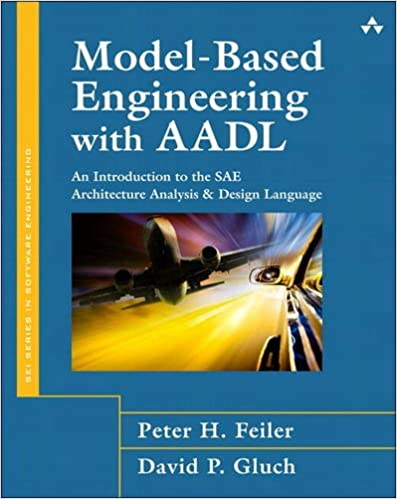
\includegraphics[width=20mm,height=28mm]{book-title-0.jpg}
\hspace*{5mm}

\includegraphics[width=20mm,height=28mm]{book-cover.jpg}


\end{frame}

\begin{frame}\frametitle{AADL in CASE}

AADL is extensible via \emph{annexes}. At Collins we have developed
two annexes used on many projects in the Trusted Systems Group:

\begin{description}
\item [AGREE] SMT-based reasoning over Assume-Guarantee contracts on components
\item [Resolute] Assurance cases as formal entities, using proof search to explore cases.
\end{description}

In CASE, AGREE is used to formulate behavioral security rqts.

Resolute is used for structural properties, and also for linking
results from disparate proof systems.

\end{frame}

\begin{frame}\frametitle{Architecture Transformations}

We have been developing a collection of architecture-to-architecture maps that can be applied to
\kemph{provably increase} the security of a system.

\vspace*{4mm}

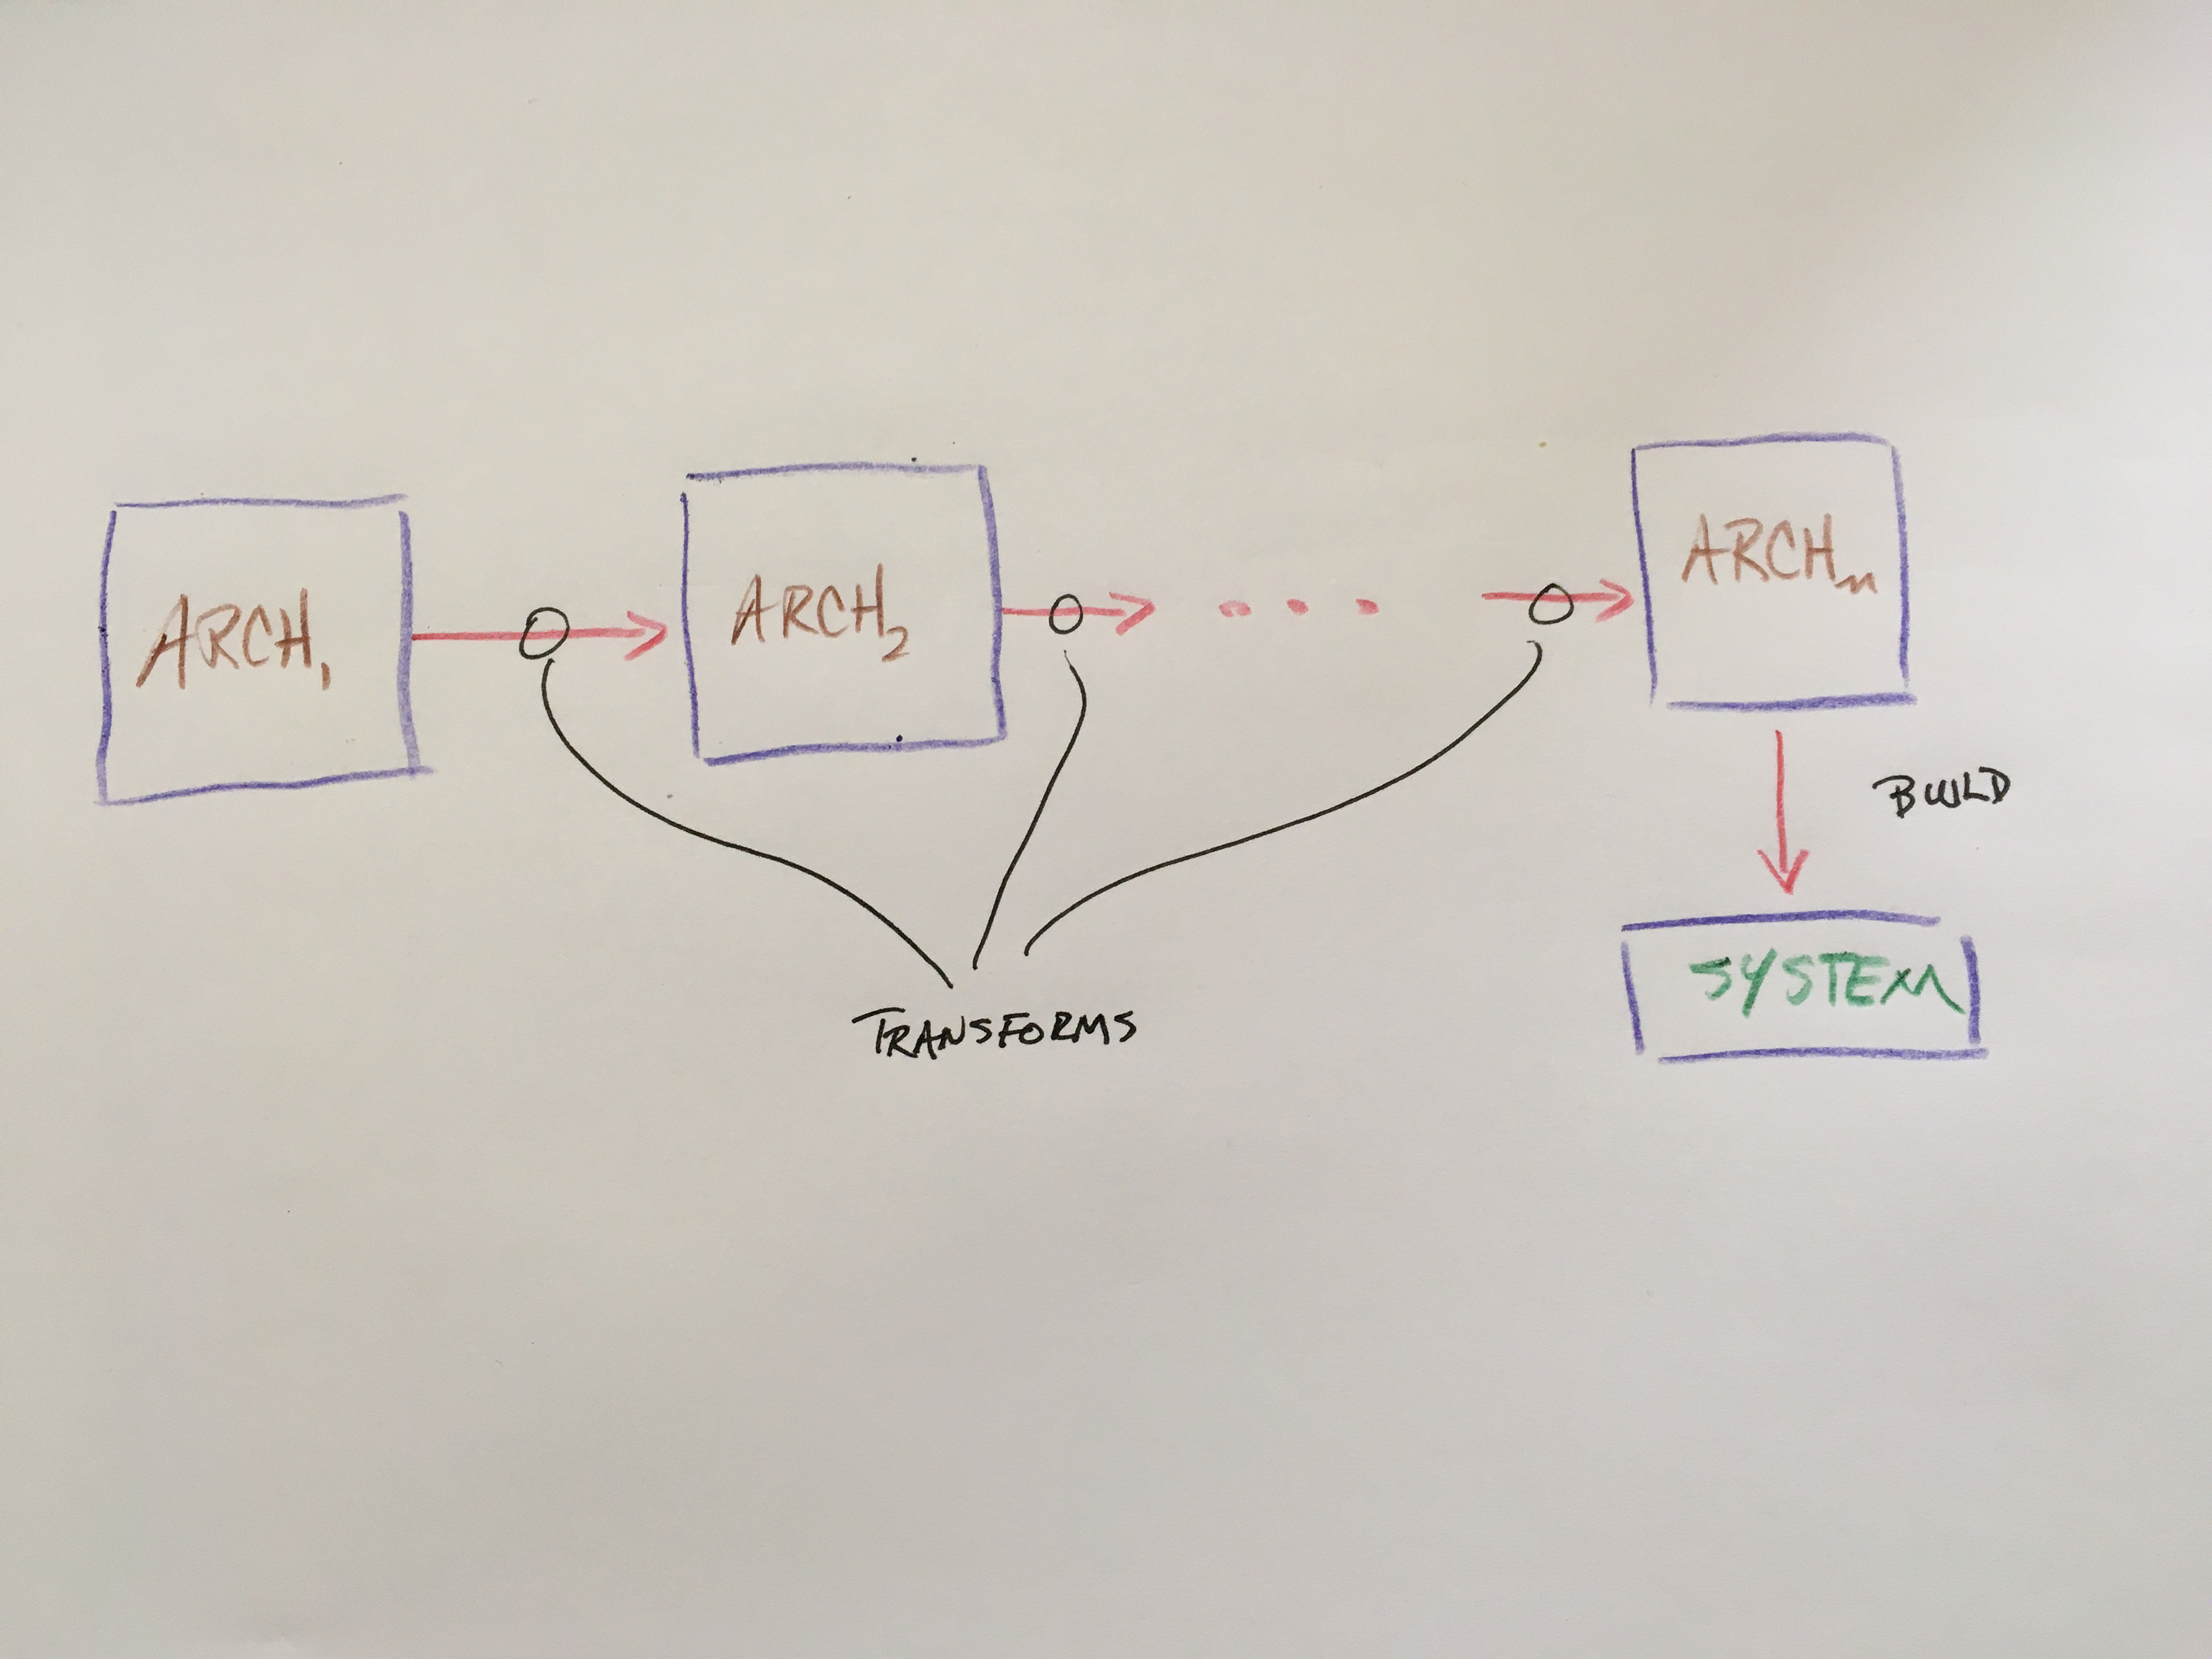
\includegraphics[width=90mm,height=50mm]{arch-trans.jpg}
\end{frame}

\begin{frame}\frametitle{Transformation: Message Filtering}

A \emph{filter} is conceptually very simple: it checks validity of its
input data according to predicate $P$.


\begin{center}
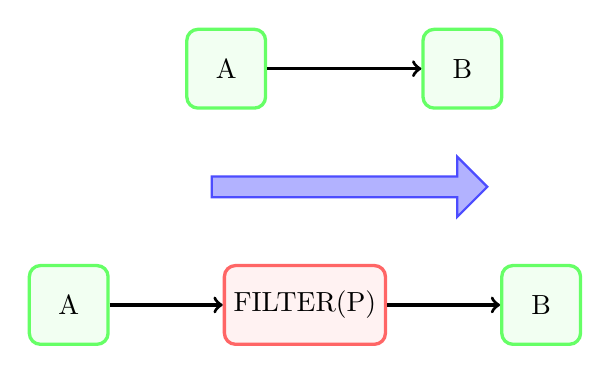
\begin{tikzpicture}[
redsquarednode/.style={rectangle, draw=red!60, fill=red!5, very thick, rounded corners, minimum size=10mm},
greensquarednode/.style={rectangle, draw=green!60, fill=green!5, very thick, rounded corners, minimum size=10mm},
fat arrow/.style={single arrow,thick,draw=blue!70,fill=blue!30,minimum height=35mm,minimum width=7mm}
]
%Nodes
\node[draw,greensquarednode] at (2,0) (SRC)    {A};
\node[draw,greensquarednode] at (5,0) (TARGET) {B};

\node at (3.5,-1.5) [fat arrow]{};

\node[draw,greensquarednode] at (0,-3) (SRC-1)    {A};
\node[draw,greensquarednode] at (6,-3) (TARGET-1) {B};
\node[draw,redsquarednode] at (3,-3) (FILTER) {FILTER(P)};

%Lines
\draw[->,very thick] (SRC.east) -- (TARGET.west);

\draw[->,very thick] (SRC-1.east) -- (FILTER.west);
\draw[->,very thick] (FILTER.east) -- (TARGET-1.west);
\end{tikzpicture}
\end{center}

%% \hspace*{10mm}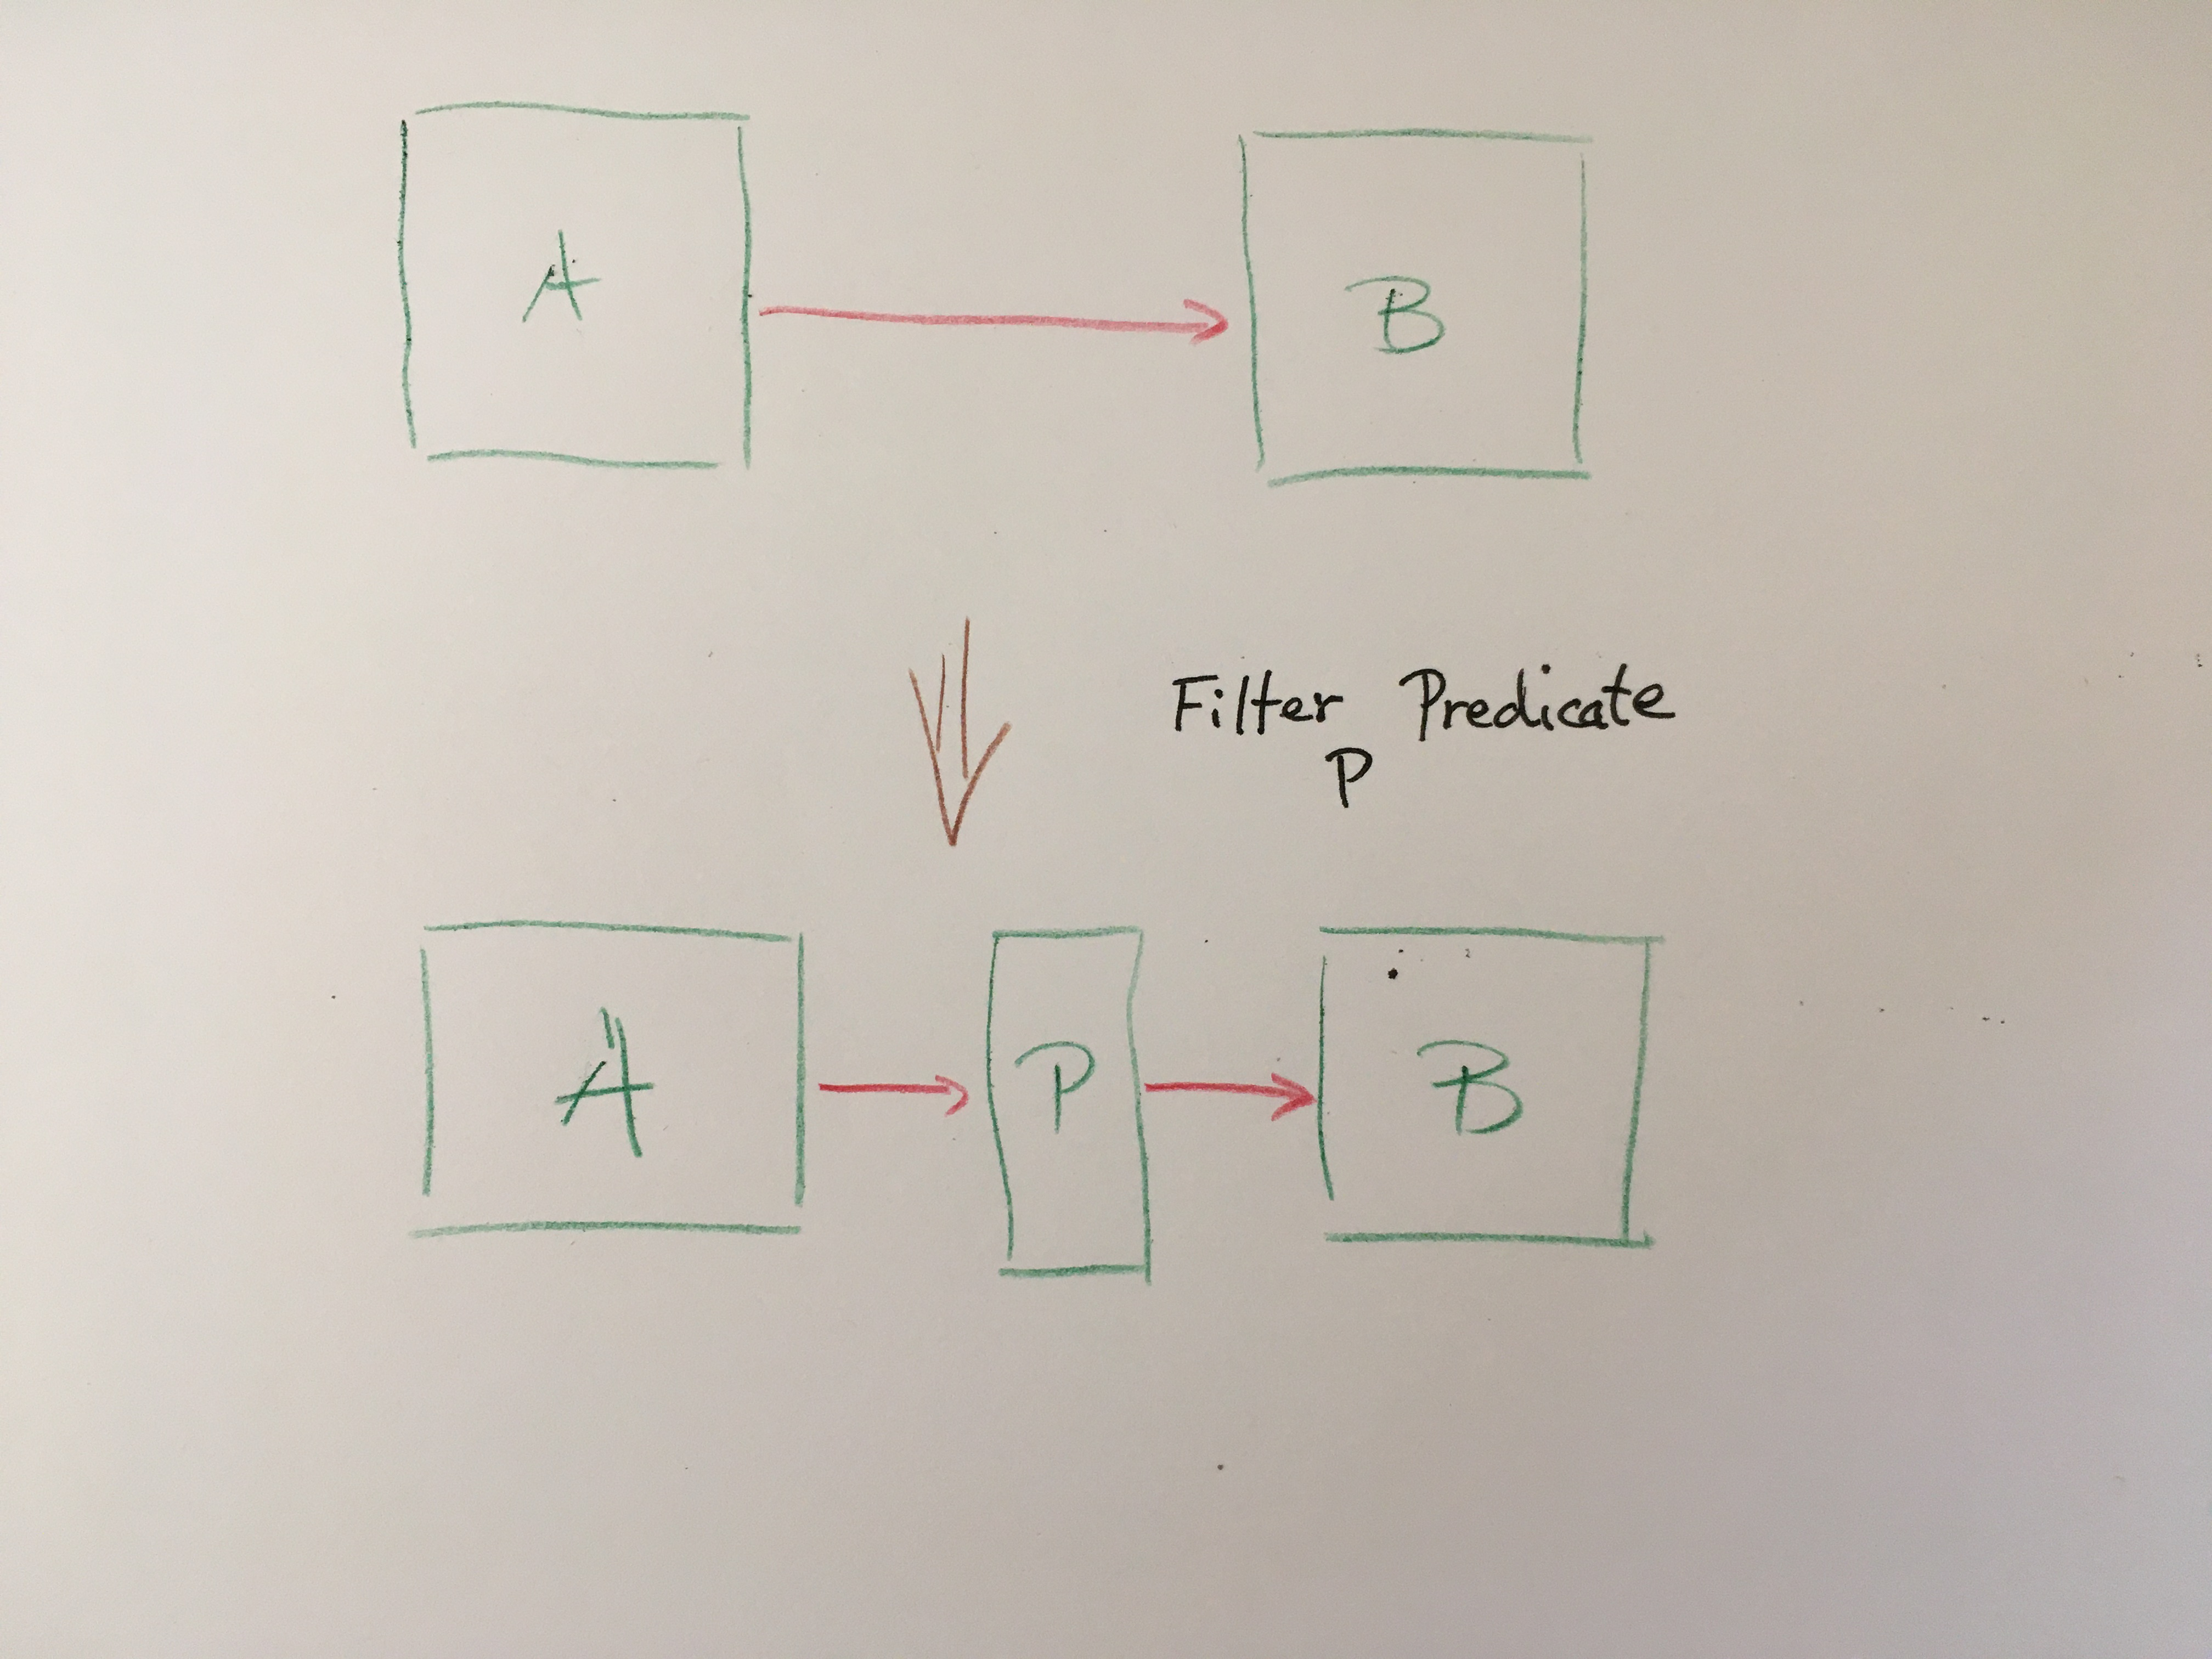
\includegraphics[width=90mm,height=50mm]{filter.jpg}

If the data is valid, then it is passed on. Otherwise it is dropped.

\end{frame}


\begin{frame}\frametitle{Transformation: Message Monitoring}

A \emph{monitor} checks to see that a relationship $\mathcal{R}$ holds
over a collection of message streams through time. If the
specification is violated, an \emph{alert} is sent out.

\begin{center}
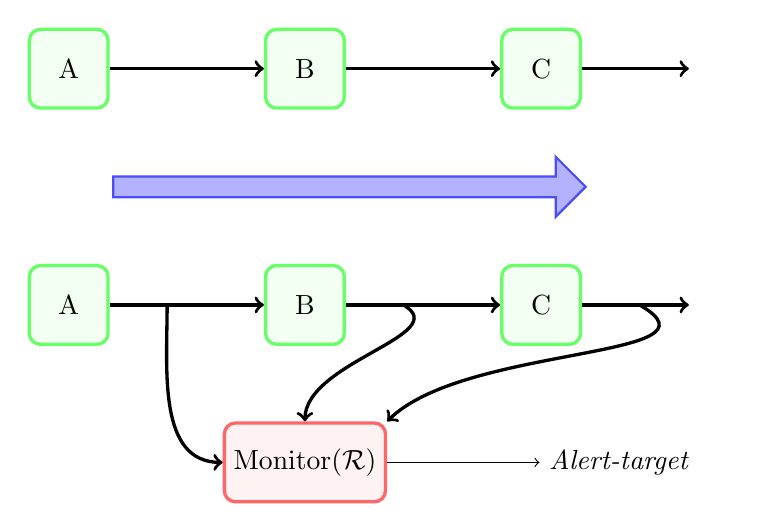
\begin{tikzpicture}[
redsquarednode/.style={rectangle, draw=red!60, fill=red!5, very thick, rounded corners, minimum size=10mm},
greensquarednode/.style={rectangle, draw=green!60, fill=green!5, very thick, rounded corners, minimum size=10mm},
fat arrow/.style={single arrow,thick,draw=blue!70,fill=blue!30,minimum height=60mm,minimum width=7mm}
]
%Nodes
\node[draw,greensquarednode] at (1,0) (A) {A};
\node[draw,greensquarednode] at (4,0) (B) {B};
\node[draw,greensquarednode] at (7,0) (C) {C};
\node at (9,0) (D) {};

\node at (4.5,-1.5) [fat arrow]{};

\node[draw,greensquarednode] at (1,-3) (A-1) {A};
\node at (2.25,-3) (joinAB) {};
\node[draw,greensquarednode] at (4,-3) (B-1) {B};
\node at (5.25,-3) (joinBC) {};
\node[draw,greensquarednode] at (7,-3) (C-1) {C};
\node at (8.25,-3) (joinCD) {};
\node at (9,-3) (D-1) {};
\node[draw,redsquarednode]   at (4,-5) (M) {Monitor($\mathcal{R}$)};
\node at (8,-5) (ALERT-TARGET) {\textit{Alert-target}};

%Lines
\draw[->,very thick] (A.east) -- (B.west);
\draw[->,very thick] (B.east) -- (C.west);
\draw[->,very thick] (C.east) -- (D.west);
\draw[->,very thick] (A-1.east) -- (B-1.west);
\draw[->,very thick] (B-1.east) -- (C-1.west);
\draw[->,very thick] (C-1.east) -- (D-1.west);

\draw[->,very thick] (2.25,-3) to [out=-90, in=180] (M);
\draw[->,very thick] (5.25,-3) to [out=-30, in=90]  (M);
\draw[->,very thick] (8.25,-3) to [out=-30, in=45]  (M.north east);
\draw[->] (M.east) -- (ALERT-TARGET);

\end{tikzpicture}
\end{center}

%% \hspace*{10mm}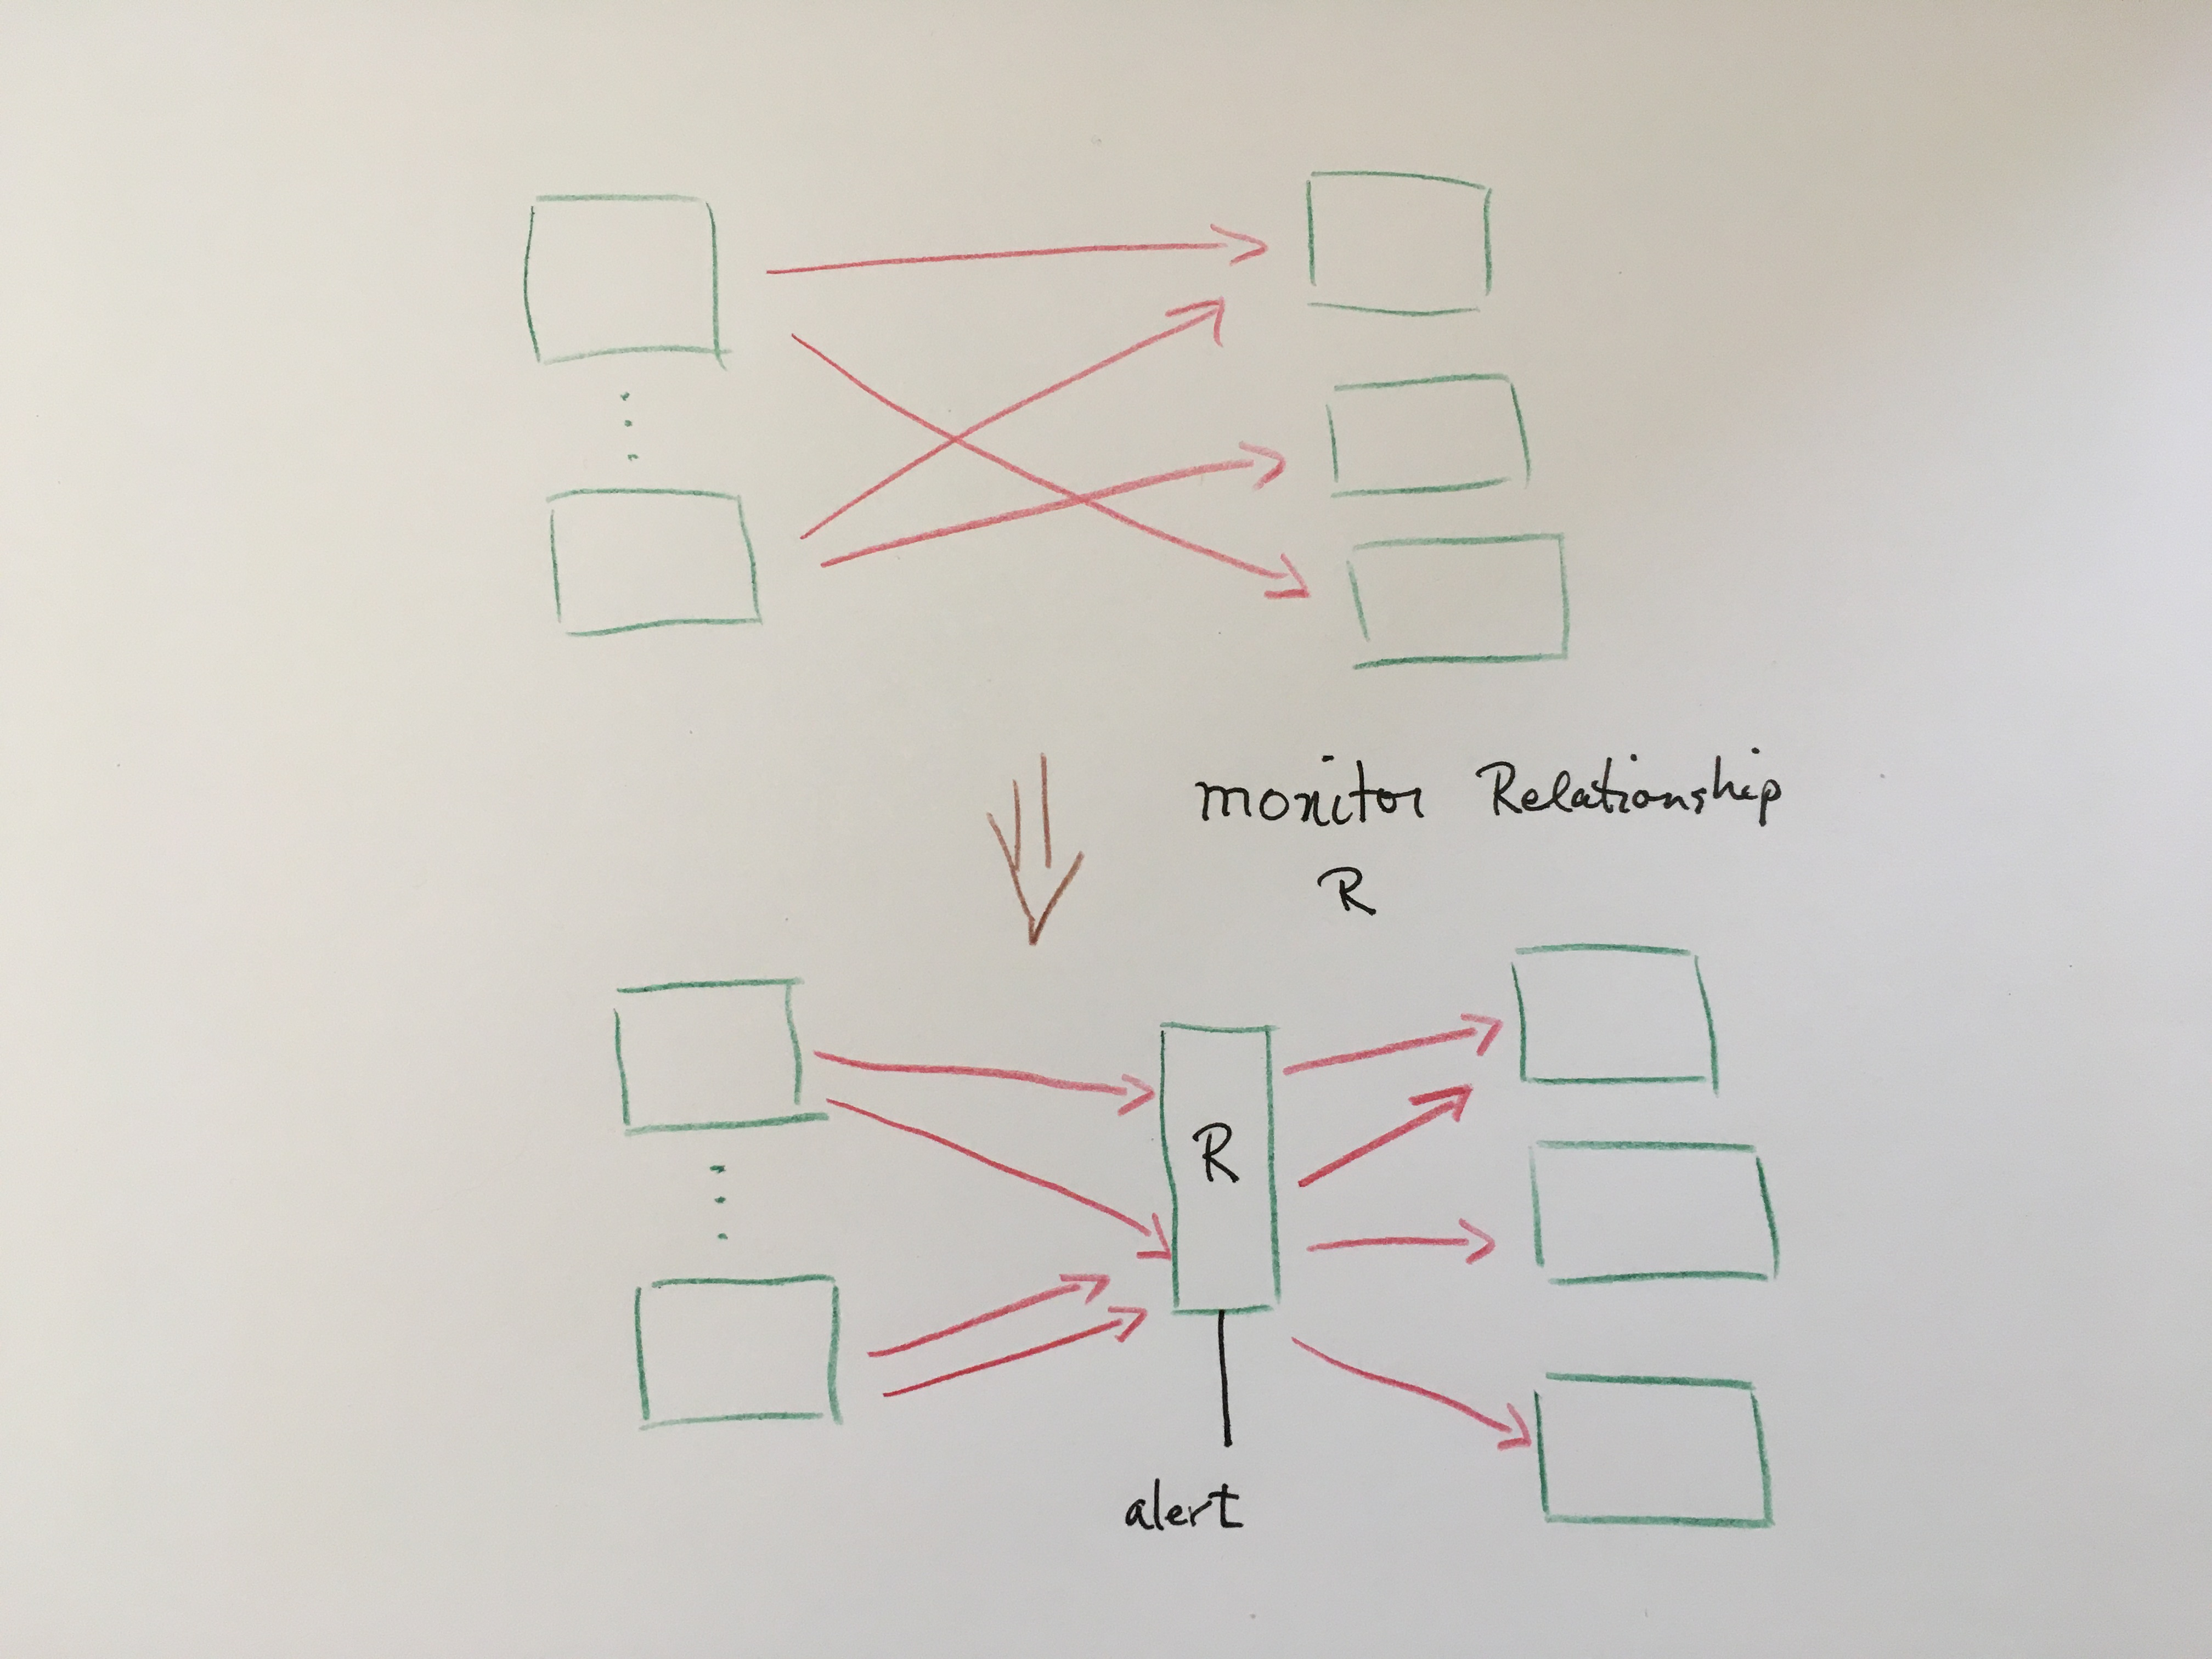
\includegraphics[width=90mm,height=40mm]{monitor.jpg}

\end{frame}

\begin{frame}\frametitle{Transformation: Message Monitoring}

  We currently use past-time temporal logic to specify monitors, following

\begin{quote}\
Efficient Monitoring of Safety Properties, Havelund and Rosu, TACAS 2002.
\end{quote}


\end{frame}


\begin{frame}\frametitle{Transformation: Isolation of `at risk' components}

An unprotected computational element can be isolated by transparently
lifting it out of its context and mediating access via seL4.

\begin{center}
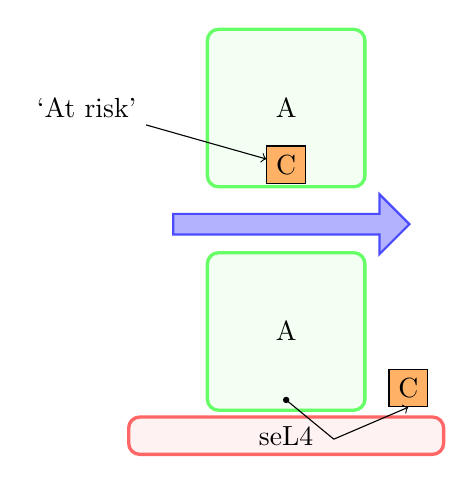
\begin{tikzpicture}[
bignode/.style =
  {rectangle,
   draw=green!60, fill=green!5,
   very thick, rounded corners,
   minimum height=20mm, minimum width = 20mm},
flatnode/.style =
  {rectangle,
   draw=red!60, fill=red!5,
   very thick, rounded corners,
   minimum width = 40mm},
fat arrow/.style={single arrow,thick,draw=blue!70,fill=blue!30,minimum height=30mm,minimum width=7mm}
]
%Nodes
\node[draw,bignode](main){A};
\node[draw,fill=orange!60] (atrisk) at ([yshift=2ex]main.south){C};
\node (comment) at ([xshift=-10ex]main.west){`At risk'};
\draw[->] (comment) -- (atrisk);
\node at ([yshift=-3ex]main.south) [fat arrow]{};
\node[draw,bignode](main-1) at ([yshift=-12ex]main.south){A};
\node[draw,fill=orange!60] (secure) at ([xshift=3.5ex,yshift=2ex]main-1.south east){C};
\node[draw,flatnode] (seL4) at ([yshift=-2ex]main-1.south){seL4};
\node[draw,fill=black,circle,scale = 0.2] (origin) at ([yshift=1ex]main-1.south){};
\node (foo) at ([yshift=-2ex,xshift=4ex]seL4.north){};
\draw (origin) -- (foo.center);
\draw[->] (foo.center) -- (secure.south);
\end{tikzpicture}
\end{center}

%\filldraw[black] (0,0) circle (2pt) node[anchor=west] {Intersection point};
%\hspace*{10mm}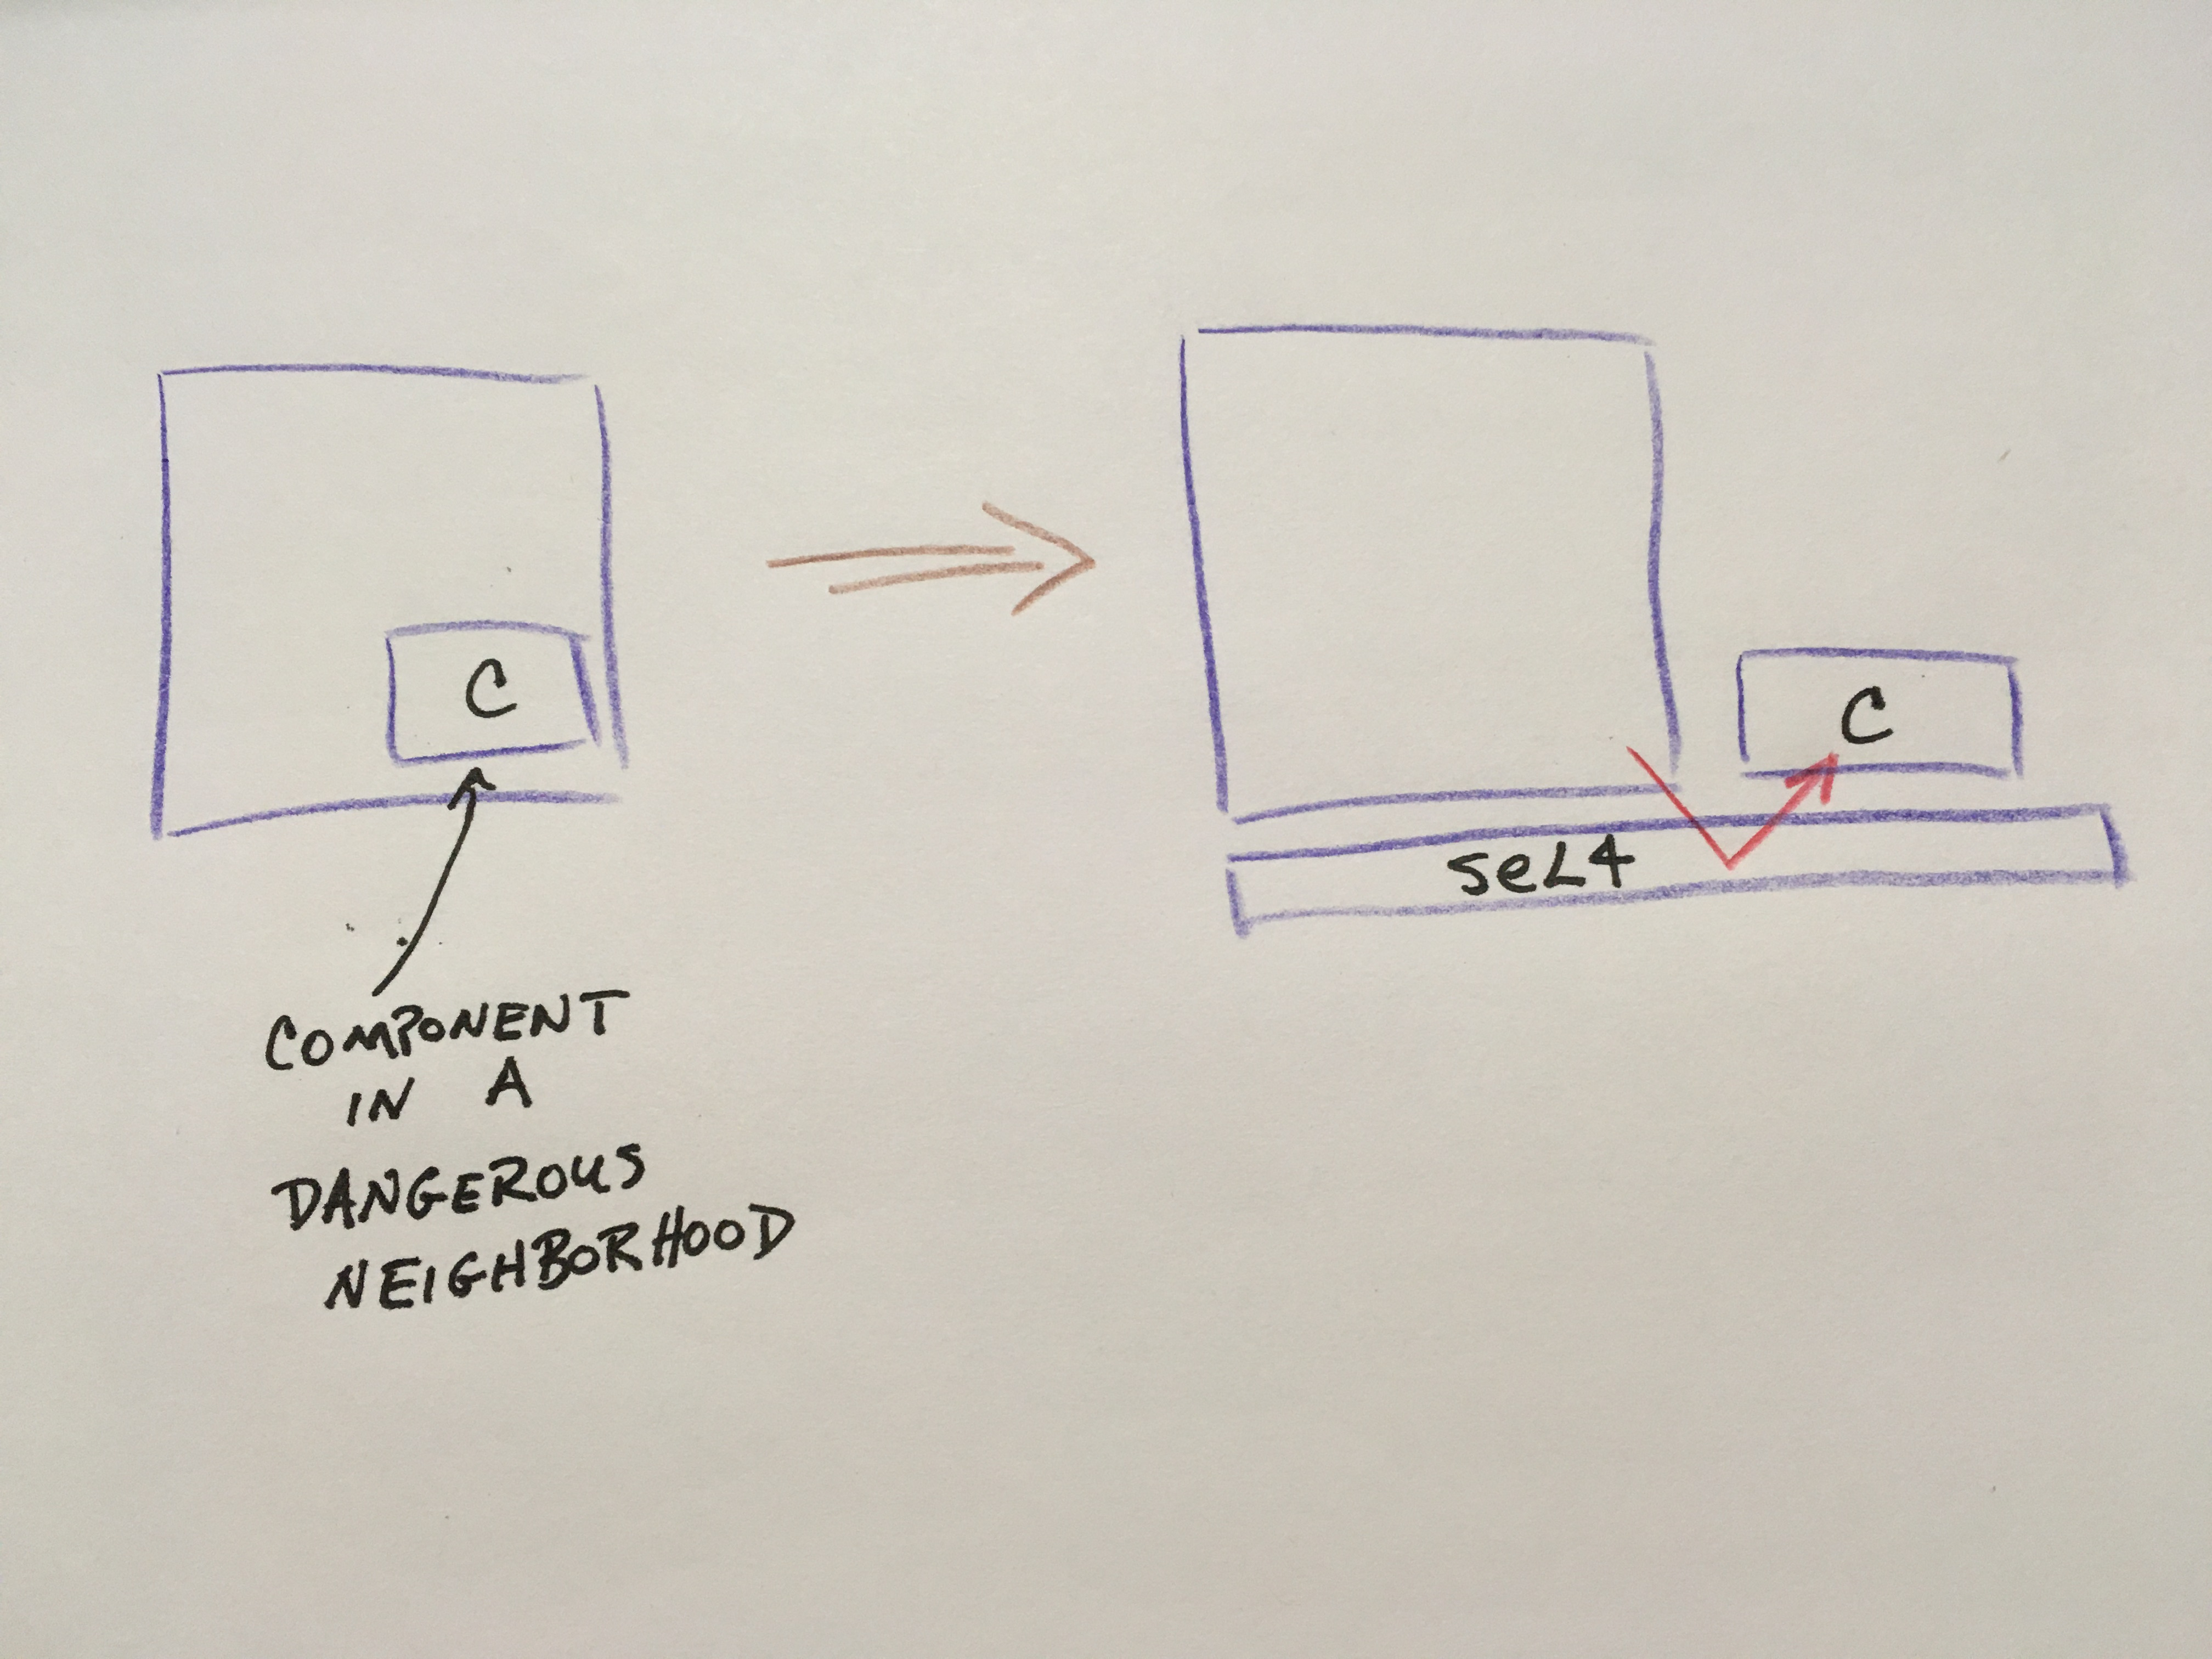
\includegraphics[width=90mm,height=40mm]{vm.jpg}

\end{frame}

\begin{frame}\frametitle{seL4}



Correctness of this transformation depends on formal guarantees provided by seL4.

\begin{itemize}
\item seL4 microkernel guarantees partitioning of components and
  communication, backed by computer-checked proofs

\item seL4 guarantees no infiltration, exfiltration, eavesdropping,
  interference, and provides fault containment for untrusted code

\end{itemize}

\vspace*{5mm}
\hspace*{10mm}
\includegraphics[width=15mm,height=15mm]{data61-logo.png}
\hspace*{10mm}
\includegraphics[width=15mm,height=15mm]{csiro--black.png}

\end{frame}

\begin{frame}\frametitle{Transformation: Attestation}

Attestation inserts measurement mechanisms into a system. These
examine various aspects of system behavior, and send summaries back to
an observer system.

\hspace*{10mm}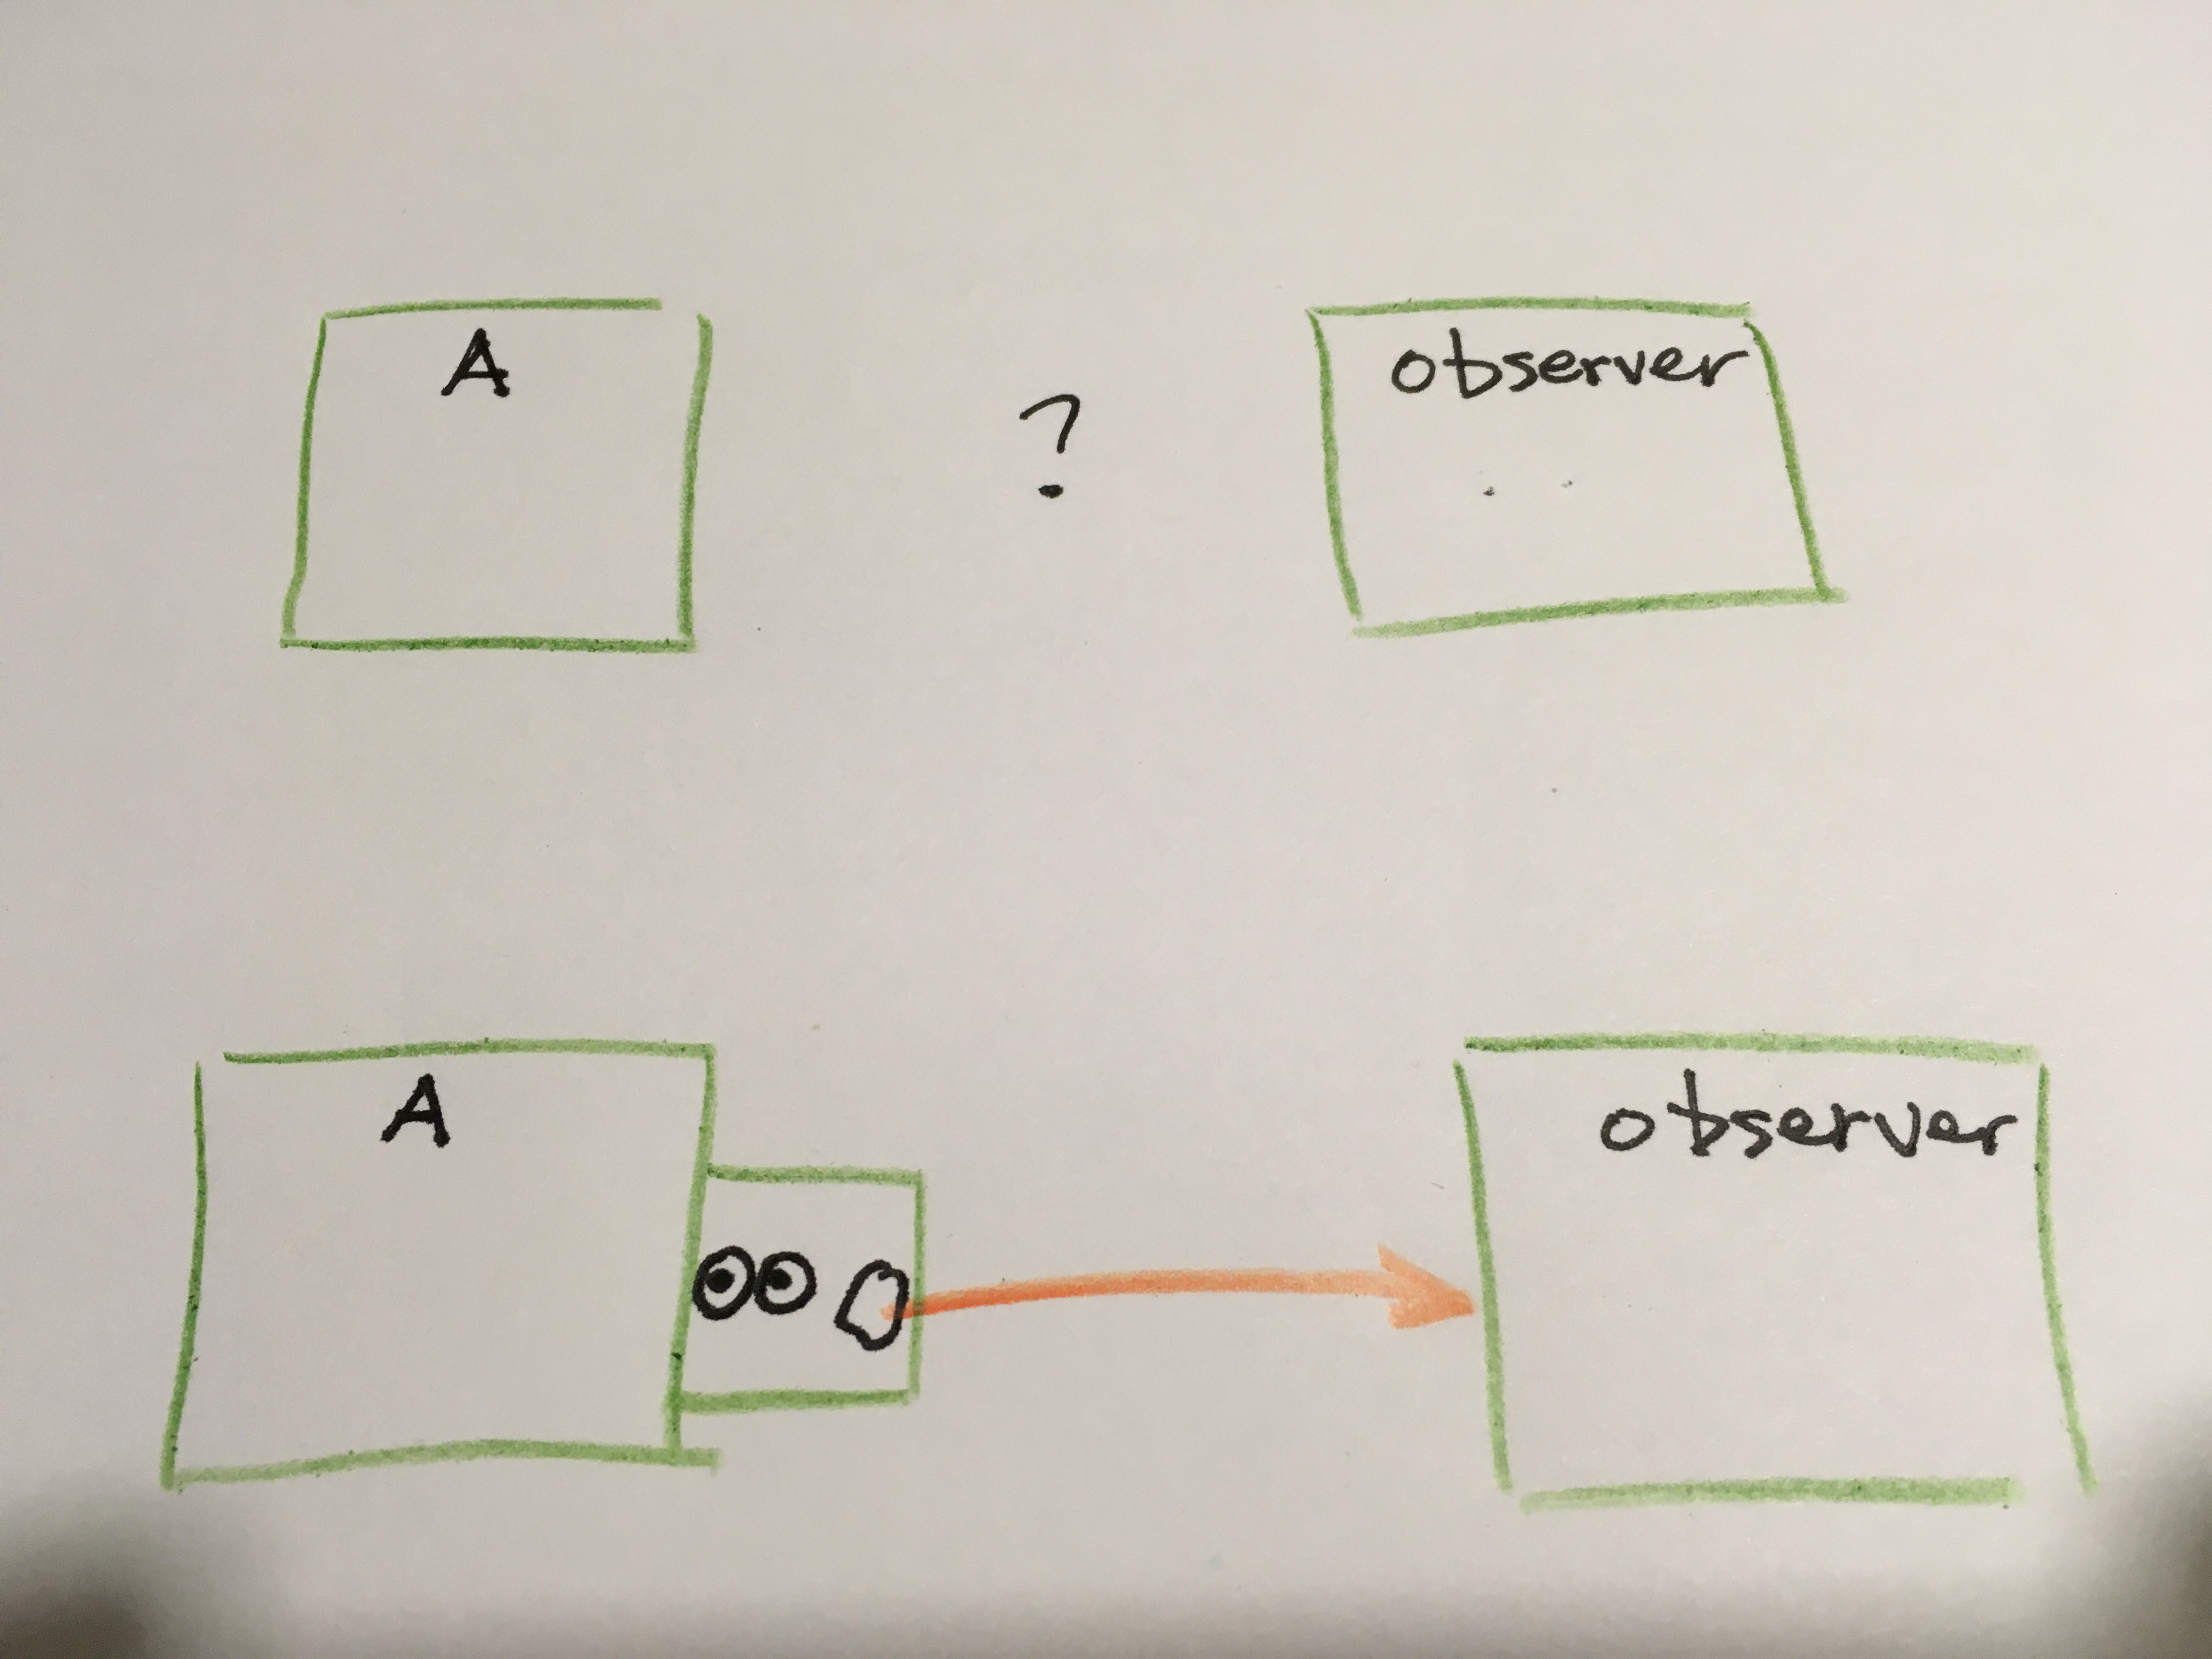
\includegraphics[width=90mm,height=40mm]{att.jpg}

\end{frame}

\begin{frame}\frametitle{CakeML connection}

  The filter, monitor, and attestation transforms generate CakeML implementations.

\begin{itemize}
 \item [$\blacktriangleright$] Currently generating source CakeML
 \item [$\blacktriangleright$] Want to generate binaries via the magic `translator` bridge between HOL and CakeML
 \item [$\blacktriangleright$] Complicated by the build process, which
   separates code generated from transform spec and the compilation
   for seL4.

\end{itemize}

\end{frame}


\begin{frame}\frametitle{Other transformations}
  This is a small but useful suite of transformations.

  There are certainly others to consider:
  \begin{itemize}
  \item encryption
  \item authentication
  \item duplicating computation + cross-checking results.
  \item etc.
  \end{itemize}

\end{frame}

\begin{frame}[fragile]\frametitle{Example System: uxAS}

 The example we have been using is \textbf{uxAS}, a framework for
 creating autonomous aerial systems from AFRL.

\begin{verbatim}
  https://github.com/afrl-rq/OpenUxAS
\end{verbatim}

\begin{itemize}
\item Open Source
\item Previous experience during the AFRL Summer of Innovation
\item Good setting in which to exercise our ideas
\end{itemize}

\end{frame}

\begin{frame}\frametitle{uxAS system architecture}

The initial system model we start from :

  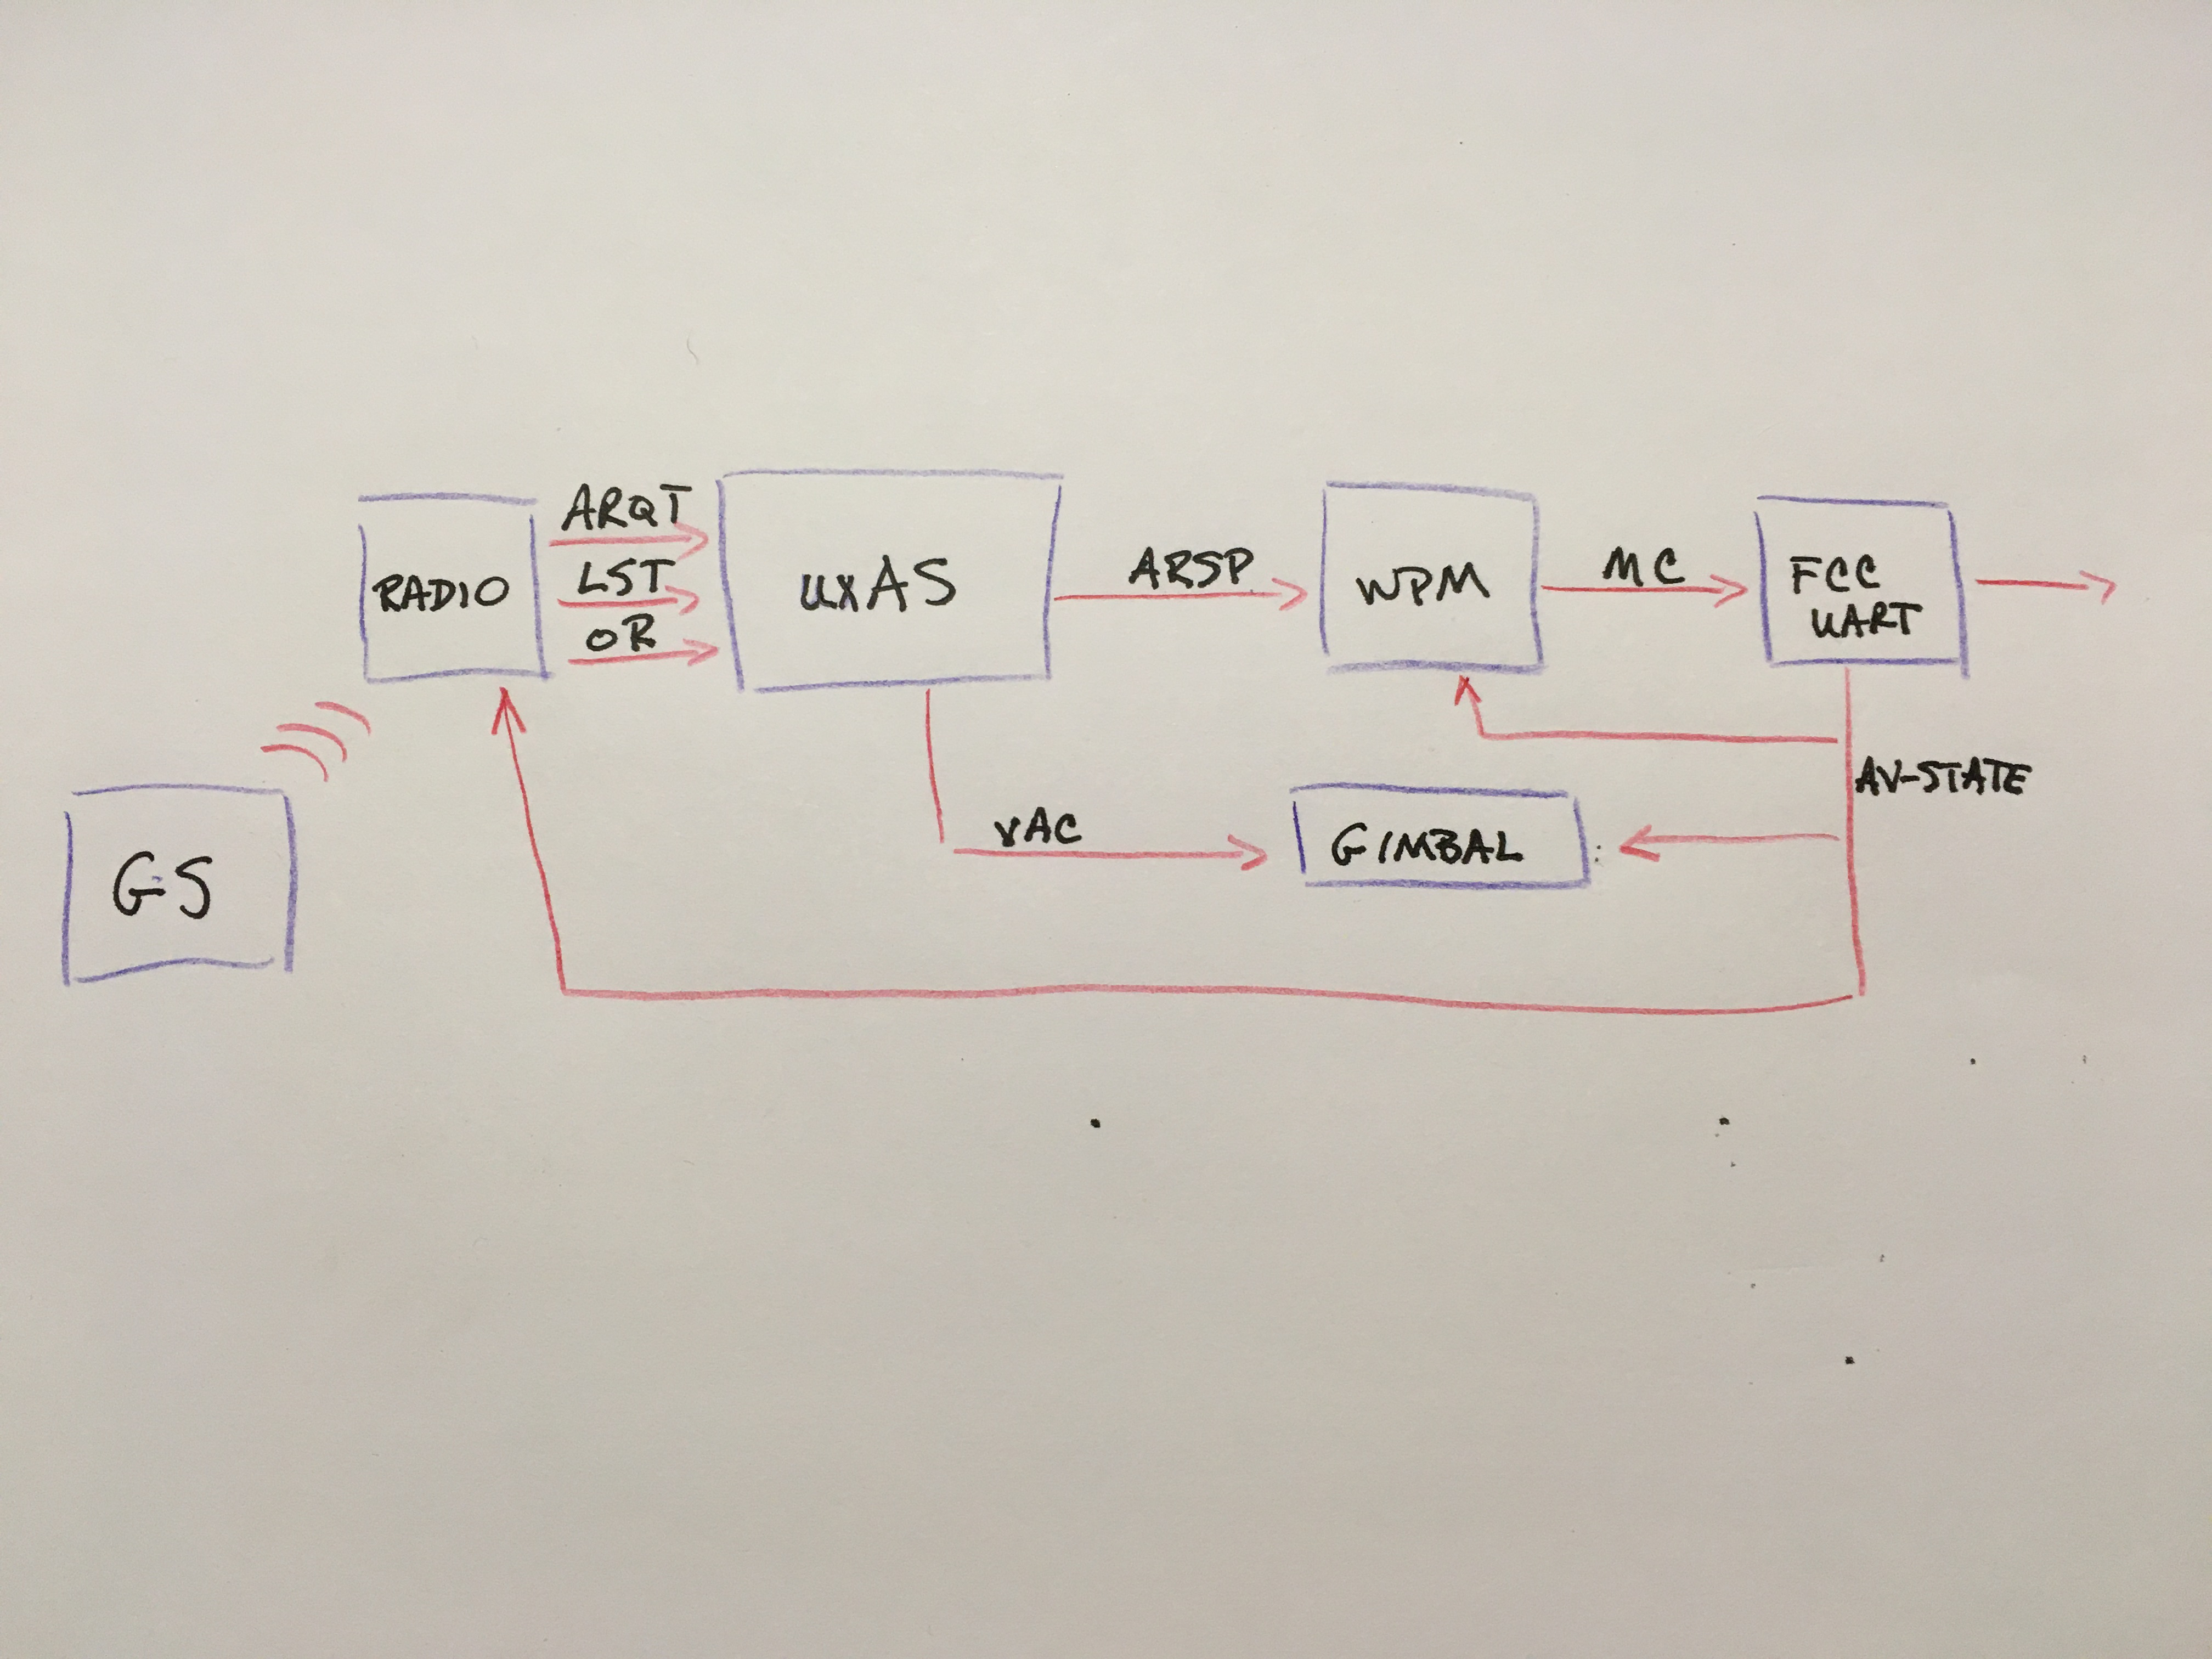
\includegraphics[width=90mm,height=50mm]{uxas-orig.jpg}


\end{frame}

\begin{frame}\frametitle{Notes on the model}

\begin{itemize}
\item UAV is preloaded with a collection of \emph{Operating Regions}
  (Keep-in and Keep-out zones)
\item Commands from GS:
\begin{description}[<+->]
  \item [OR] Set operating region
  \item [LST] LineSearchTask: \colorbox{orange}{Follow the given sequence of points}
  \item [ARQT] : AutomationRequest: \colorbox{orange}{Create a flight plan to
    achieve a high-level description,}
\colorbox{orange}{e.g., ``surveil the given OR in a grid pattern''}
\end{description}

\item Internal messages
\begin{description}
  \item [ARSP]  Response to Automation Request
  \item [VAC]  VehicleActionCommand
  \item [MC]  MissionCommand
  \item [AV-State] AirVehicleState
\end{description}

\end{itemize}

\end{frame}

\begin{frame}\frametitle{Security Considerations}

\begin{itemize}[<+->]
\item \colorbox{red}{\textbf{Problem}} An Operating Region message should designate a known region
\item \colorbox{green}{\textbf{Solution}} Filter OR message to be valid regions

\item \colorbox{red}{\textbf{Problem}} Each point in a Line Search Task should be a valid GPS coordinate
\item \colorbox{green}{\textbf{Solution}} Filter LST message on GPS coords

\item \colorbox{red}{\textbf{Problem}} Each point in an Automation Response should be
  in a keep-in zone and not in a keep-out zone
\item \colorbox{green}{\textbf{Solution}} Monitor ARSP messages wrt Keep-in and Keep-out zones

\item \colorbox{red}{\textbf{Problem}}: Every point in an Automation Response should be a valid GPS coord
\item \colorbox{green}{\textbf{Solution}} Filter ARSP message
\end{itemize}

\end{frame}

\begin{frame}\frametitle{Security Considerations continued}

\begin{itemize}[<+->]
\item \colorbox{red}{\textbf{Problem}} Every Automation Request should have a corresponding Response
\item \colorbox{green}{\textbf{Solution}} Monitor ARQT and ARSP for responses matching requests

\item \colorbox{red}{\textbf{Problem}}: uxAS software is open source and Waypoint Manager could be compromised
\item \colorbox{green}{\textbf{Solution}} Isolate Waypoint Manager on a VM

\item \colorbox{red}{\textbf{Problem}}: Ground station could be compromised; UAV needs to defend itself against that
\item \colorbox{green}{\textbf{Solution}} Attestation Manager on GS, observing activity
  on the GS and talking to UAV
\end{itemize}

\end{frame}


\begin{frame}\frametitle{Transformed uxAS}

The transformed model :

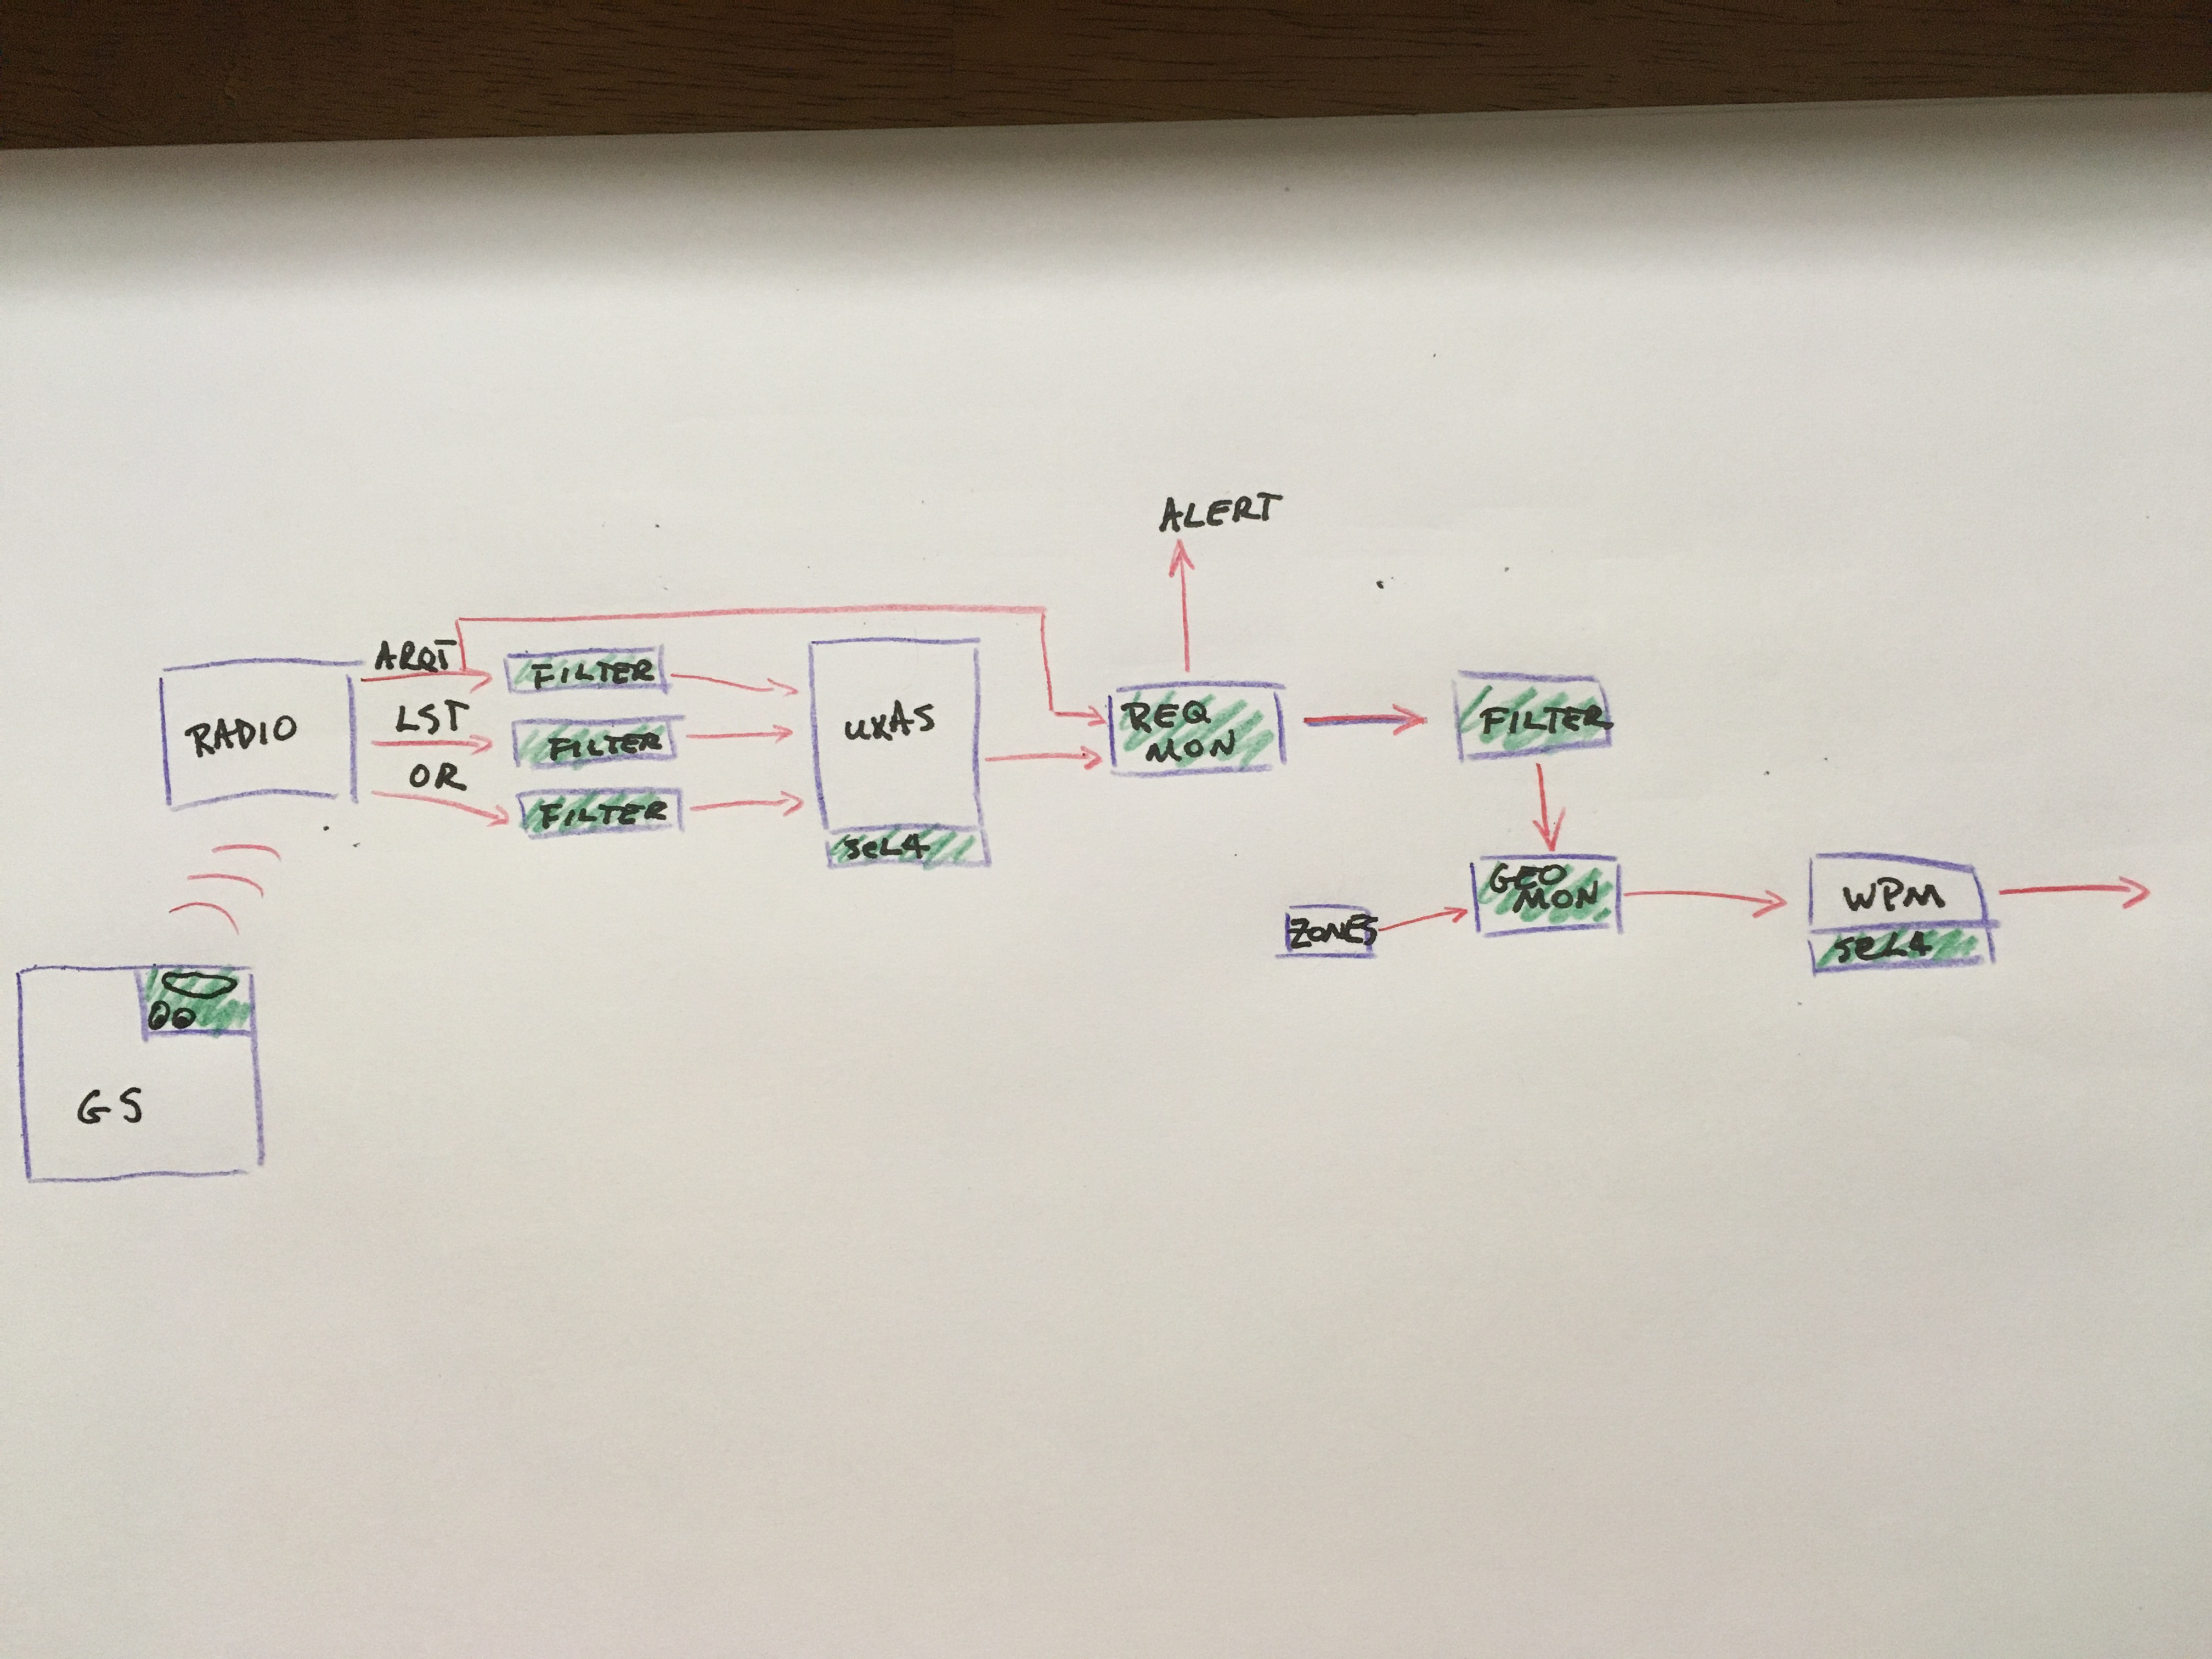
\includegraphics[width=90mm,height=50mm]{final-arch.jpg}

\end{frame}

\begin{frame}\frametitle{Implementations and Build}

As the transformations are applied, implementations and
configuration information are generated.

\begin{itemize}

  \item For ``simple'' transformations code can be generated at transformation time.
  \item For the VM and Attestation transforms, configuration
    information can be generated, but the details of the
    implementation are more involved.
\end{itemize}

Finally the \textbf{BUILD} can now be invoked.


\includegraphics[width=20mm,height=20mm]{ksu.jpg}

\includegraphics[width=20mm,height=20mm]{adventium.png}


\end{frame}

\begin{frame}\frametitle{Build}

The build is very challenging. The \textbf{HAMR} toolsuite implements
multi-stage translation architecture to address the following goals:
\begin{itemize}

\item Semantic consistency from model to execution ensures model-level
  analysis applies to deployed code

\item Build for multiple target platforms: seL4, Linux

\item Same computational model across different platforms

\item Same semantics for threading and communication

\end{itemize}

\end{frame}

\begin{frame}[fragile]\frametitle{Summary}

System designer uses OSATE, using menus to specify and configure transforms.

The interface makes sanity checks and sets up for the eventual system build

For a nice video on the interface see
\begin{verbatim}
  http://loonwerks.com/projects/case.html
\end{verbatim}

\end{frame}

\section {Deep Dive: Message Filters}

\begin{frame}\frametitle{Solutions lead to new problems}

Once implementations are created for the new system components, we
have to guard against \kemph{increasing the attack surface} of the system.

Formal specification and proof to the rescue!

\end{frame}

\begin{frame}\frametitle{Ports and messages}

Question: what does a filter operate over?

\begin{itemize}

  \item An AADL component communicates with other components via \kemph{typed connections}

\item  Types are the usual finite types from programming: booleans,
  integers, floats, arrays, records, unions, etc.

\item Properties in AGREE (our specification language) are therefore
  written over these types.

\item In particular, the `add-a-filter' transform is specified by a predicate over the input port type.

\end{itemize}

\end{frame}

\begin{frame}[fragile]\frametitle{Example : Wellformed GPS coordinates in AGREE}

{\small
\begin{verbatim}
 AltitudeType = AGL | MSL

 Location3D = {
  Latitude  : real64,
  Longitude : real64,
  Altitude  : real32,
  AltitudeType : AltitudeType}

 Good_Location (loc) =
    -90.0 <= loc.Latitude <= 90.0 and
   -180.0 <= loc.Longitude <= 180.0 and
      0.0 <= loc.Altitude <= 15000.0
\end{verbatim}
}

\end{frame}

\begin{frame}\frametitle{Example : Wellformed GPS strings}

However, in the implementation, messages coming into a port are
byte arrays (essentially untyped).

\[
\begin{array}{l}
 \konst{Good\_Location\_Mesg} (s) \iff \\
\quad   \exists s_1 s_2 s_3 s_4. \\
\qquad      s = s_1 \bullet s_2 \bullet s_3 \bullet s_4 \ \land \\
\qquad    -90.0 \leq \konst{doubleVal}(s_1) \leq 90.0 \ \land \\
\qquad   -180.0 \leq \konst{doubleVal}(s_2) \leq 180.0 \ \land \\
\qquad      0.0 \leq \konst{floatVal}(s_3)  \leq 15000.0 \ \land \\
\qquad        0 \leq \konst{natVal}(s_4) \leq 1
\end{array}
\]
%
\noindent where
%
\[
\begin{array}{ll}
 \konst{doubleVal} & : \konst{string} \to \konst{double} \\
 \konst{floatVal}  & : \konst{string} \to \konst{float}  \\
 \konst{natVal}    & : \konst{string} \to \konst{nat}  \\
\end{array}
\]

\end{frame}

\begin{frame}\frametitle{SPLAT}

We need to span the gap between specifications on high level data and
implementations over flat strings.

Our approach : \kemph{\textbf{SPLAT}} (Semantic Properties for Language and Automata Theory)

Try to apply ideas from Formal Language Theory to showing properties
of operations on high-level data.

\end{frame}

\begin{frame}[fragile]\frametitle{SPLAT the early days}

Initial version of SPLAT was based on HOL4 library of regexps developed with Scott Owens.

\begin{itemize}[<+->]
\item [$\blacktriangleright$] Regard a message as a concatenation of \emph{fields}
\item [$\blacktriangleright$] Each field has an interval spec of the form $\mathit{lo} \leq \mathit{field} \leq \mathit{hi}$
\item [$\blacktriangleright$] An interval spec can be translated to a regexp which is a
  predicate on the binary representation of the field.
\item The concatenation of regexps for the message fields gives a big regexp for the message.
\item [$\blacktriangleright$] Filter is obtained by compiling (via bespoke \konst{EVAL}) regexp to DFA.
\item [$\blacktriangleright$] Worked example by Johannes in CakeML distrib: \verb+examples/filterProgScript.sml+
\end{itemize}

\end{frame}

\begin{frame}[fragile]\frametitle{Self-describing messages}

Unfortunately, many message formats can't be captured by regexps.

Message formats commonly have \kemph{self-describing} aspects such as

\begin{itemize}
\item \kemph{length} fields, which represent sizes for other parts of the message, e.g., a list of elements, paired with its length
\item \kemph{unions}, which allow multiple versions of a format to exist in a single format, e.g.
  \textit{If field A is less than 14 then the message has 10 fields, else it has 15}
\end{itemize}

In combination these features can lead to tricky formats.

Such self-describing aspects can't be handled properly with regular or context-free languages. Maybe context-sensitive langs would work but I hear they are hopeless.


\end{frame}

\begin{frame}[fragile]\frametitle{Example: uxAS LineSearchTask messages}

\begin{description}
  \item [TaskID] \verb+i64+, basic type
  \item [Label] \verb+vString+, variable-length string
  \item [EligibleEntities] \verb+BoundedArray i64 32+, \\
    variable length array of ints, length max 32.
  \item [Parameters] \verb+BoundedArray keyValuePair_Option 8+, \\
variable length array of optional pairs of \verb+vString+, max size 8.

  \item [PointList] \verb+ BoundedArray location3D_Option 1024+, \\

  \item [etc]
\end{description}

\end{frame}

\begin{frame}[fragile]\frametitle{Contiguity types}

We specify message formats using \kemph{contiguity types}. With this
representation we can automatically

\begin{itemize}
\item generate verified message filters (and parsers)

\item generate random test messages

\item prove that the message-level filter has the specfied representation-level property
  (\verb+Good_Location_Mesg+ in our example)

\end{itemize}

%% The goal is to automatically generate an implementation of the
%% well-formedness predicate \verb+Good_Location+ from its specification.

%% There is a problem : the encoding from datastructures to strings is not specified.

%% For uxAs, this is a fairly complex encoding.
\end{frame}


\begin{frame}[fragile]\frametitle{Contiguity types: syntax}

The syntax of contiguity types is very similar to a standard
collection of base types closed under formation of records and arrays.

\[
\begin{array}{rcl}
 \mathit{base} & = & \konst{bool} \mid \konst{char} \mid \konst{u8} \mid
 \konst{u16} \mid \konst{u32} \mid \konst{u64}  \mid \konst{i16} \mid
 \konst{i32} \mid \konst{i64} \mid \konst{f32} \mid \konst{f64} \\
 \tau & = & \mathit{base} \\
      & \mid & \konst{Recd}\; (f_1 : \tau_1) \ldots (f_n : \tau_n) \\
      & \mid & \konst{Array}\; \tau \; \mathit{exp} \\
      & \mid & \konst{Union}\; (\mathit{bexp}_1 : \tau_1) \ldots (\mathit{bexp}_n : \tau_n)
\end{array}
\]
\end{frame}

\begin{frame}[fragile]\frametitle{Contiguity types: examples}
\end{frame}

\begin{frame}[fragile]\frametitle{Contiguity types: semantics}

The semantics of contiguity types is in terms of formal languages
(sets of strings):

\[
% \begin{array}{l}
\LangTheta{\tau} =
\mathtt{case}\; \tau\
% \hspace*{3mm}
 \left\{
 \begin{array}{l}
 \mathit{base} \Rightarrow \set{s \mid \konst{len}(s) = \konst{width}(base)} \\
 \konst{Recd}\; (f_1 : \tau_1) \ldots (f_n : \tau_n)
      \Rightarrow \LangTheta{\tau_1} \cdot \ldots \cdot \LangTheta{\tau_n}
\\
 \konst{Array}\; \tau_1 \; \mathit{exp}
      \Rightarrow  \LangTheta{\tau_1}^{\konst{evalExp}\;\theta\;\mathit{exp}}
\\
 \konst{Union}\; (\mathit{bexp}_1 : \tau_1) \ldots (\mathit{bexp}_n : \tau_n) \Rightarrow \\
  \hspace*{5mm}
 \left\{
 \begin{array}{ll}
    \LangTheta{\tau_i} &  \mathrm{if}\ \konst{evalBexp}\;\theta\;\mathit{bexp}_i = \konst{true} \\
                  & \mathrm{and\ no\ other}\ \mathit{bexp}_j\ \mathrm{is}\ \konst{true}  \\
    \emptyset & \mathrm{otherwise}
 \end{array}
 \right.
 \\
\end{array}
 \right.
%\end{array}
\]
\end{frame}

\begin{frame}[fragile]\frametitle{Correctness of parameterized matcher}

We can define a function \textbf{match} which takes a contig type and
a string and returns an assignment of slices of the string to elements of the type.

\begin{theorem}[Soundness]
  \[
 \vdash \konst{match}\; \mathit{contig}\; \mathit{string} = \konst{Some}(\theta) \imp
   \mathit{string} \in \LangTheta{\mathit{contig}}
\]
\end{theorem}

\textbf{match} has the flavor of a \kemph{parser generator}: it takes a
specification of the language to be parsed and returns an implementation

\colorbox{orange}{We use \textbf{match} to implement all filters in
  the transformed uxAS.}

\end{frame}

\begin{frame}[fragile]\frametitle{Assert types}
\end{frame}

\begin{frame}\frametitle{Yet to be done}

\begin{itemize}
\item incorporating decoder and encoder to close the gap with the type-level specs
\item completeness proof
\item symbolic evaluation of a contig-type in the semantics
\item compiling contig-types into fast copy-free implementations
\item comparison with dependent type approach
\end{itemize}
\end{frame}


\begin{frame}\frametitle{CakeML compiler comments}

CakeML has fit into the CASE development process pretty well!

\begin{itemize}
\item compiles 1200-odd line programs reasonably fast
\item FFI simple and easy to work with
\item library is small but fairly complete for my purposes
\item resulting code compiles in with C just fine
\item no surprises
\item BUT: needs docs and improved front-end syntax error messages
\end{itemize}
\end{frame}

\begin{frame}\frametitle{Joining theorems together}

  We can join the correctness of the message matcher with the
  correctness of the CakeML toolchain to obtain a \kemph{single-shot}
  correctness theorem in HOL4:
  \vspace*{5mm}

  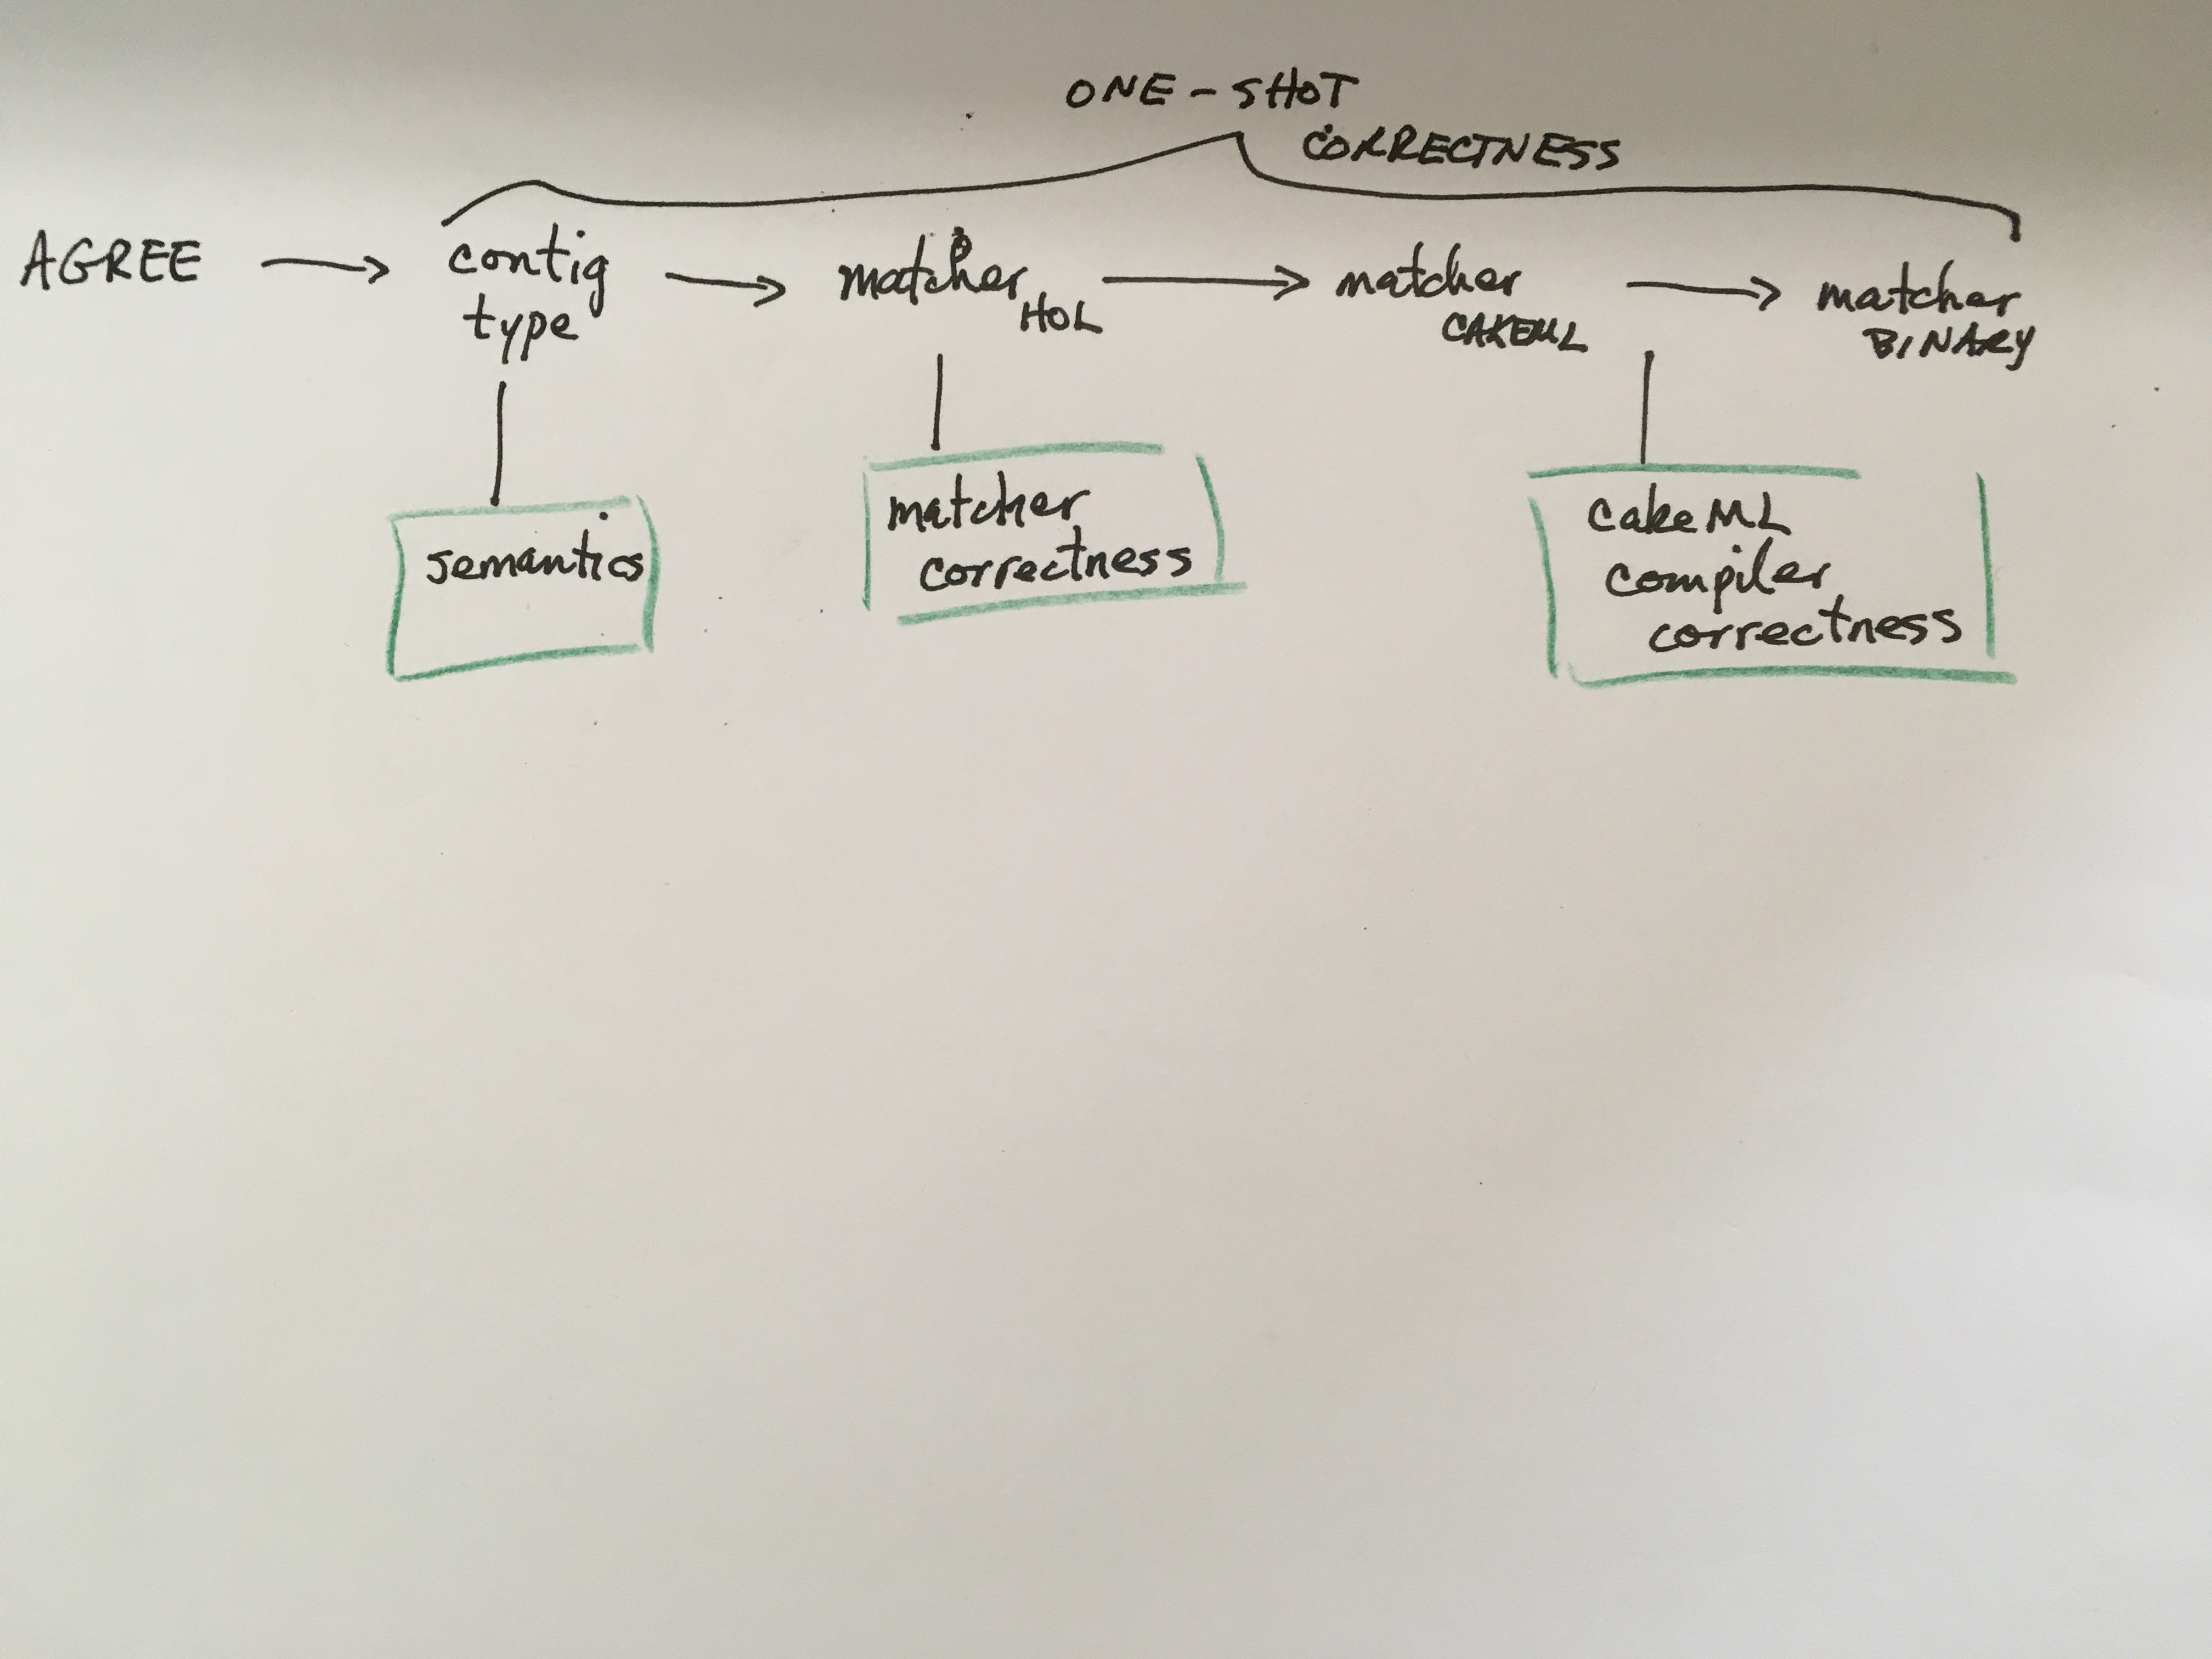
\includegraphics[width=90mm,height=50mm]{one-shot.jpg}

\end{frame}

\begin{frame}\frametitle{Question: value of end-to-end verification}

Q: What is the value of combining verified programs with a verified
   compiler to get a property of the compiled program?

A: It removes places to look for bugs. Instead, the assumptions of the
final joined-up theorem reveal the limitations on applicability of the
result.

A: [John Matthews] It's a formal verification version of system test:
checks that all pre-and-post conditions fit together properly

\end{frame}


\begin{frame}[fragile]\frametitle{Thread level correctness}

But we need to do better: the filter is run inside a loop:

{\small
\begin{verbatim}
  while true
  do {
    getInput();
    if match contig inputBuf {
      putOutput (inputBuf);
     }
    else skip;
   }
\end{verbatim}
}
\end{frame}

\begin{frame}[fragile]\frametitle{Thread level correctness}

Thanks to some great work from Johannes {\AA}man Pohjola at Data61
(and others in the CakeML gang) we can think about proving the
correctness at the thread level:

\begin{itemize}
\item proof rules for infinitary computations with I/O
\item space bounds proofs
\end{itemize}

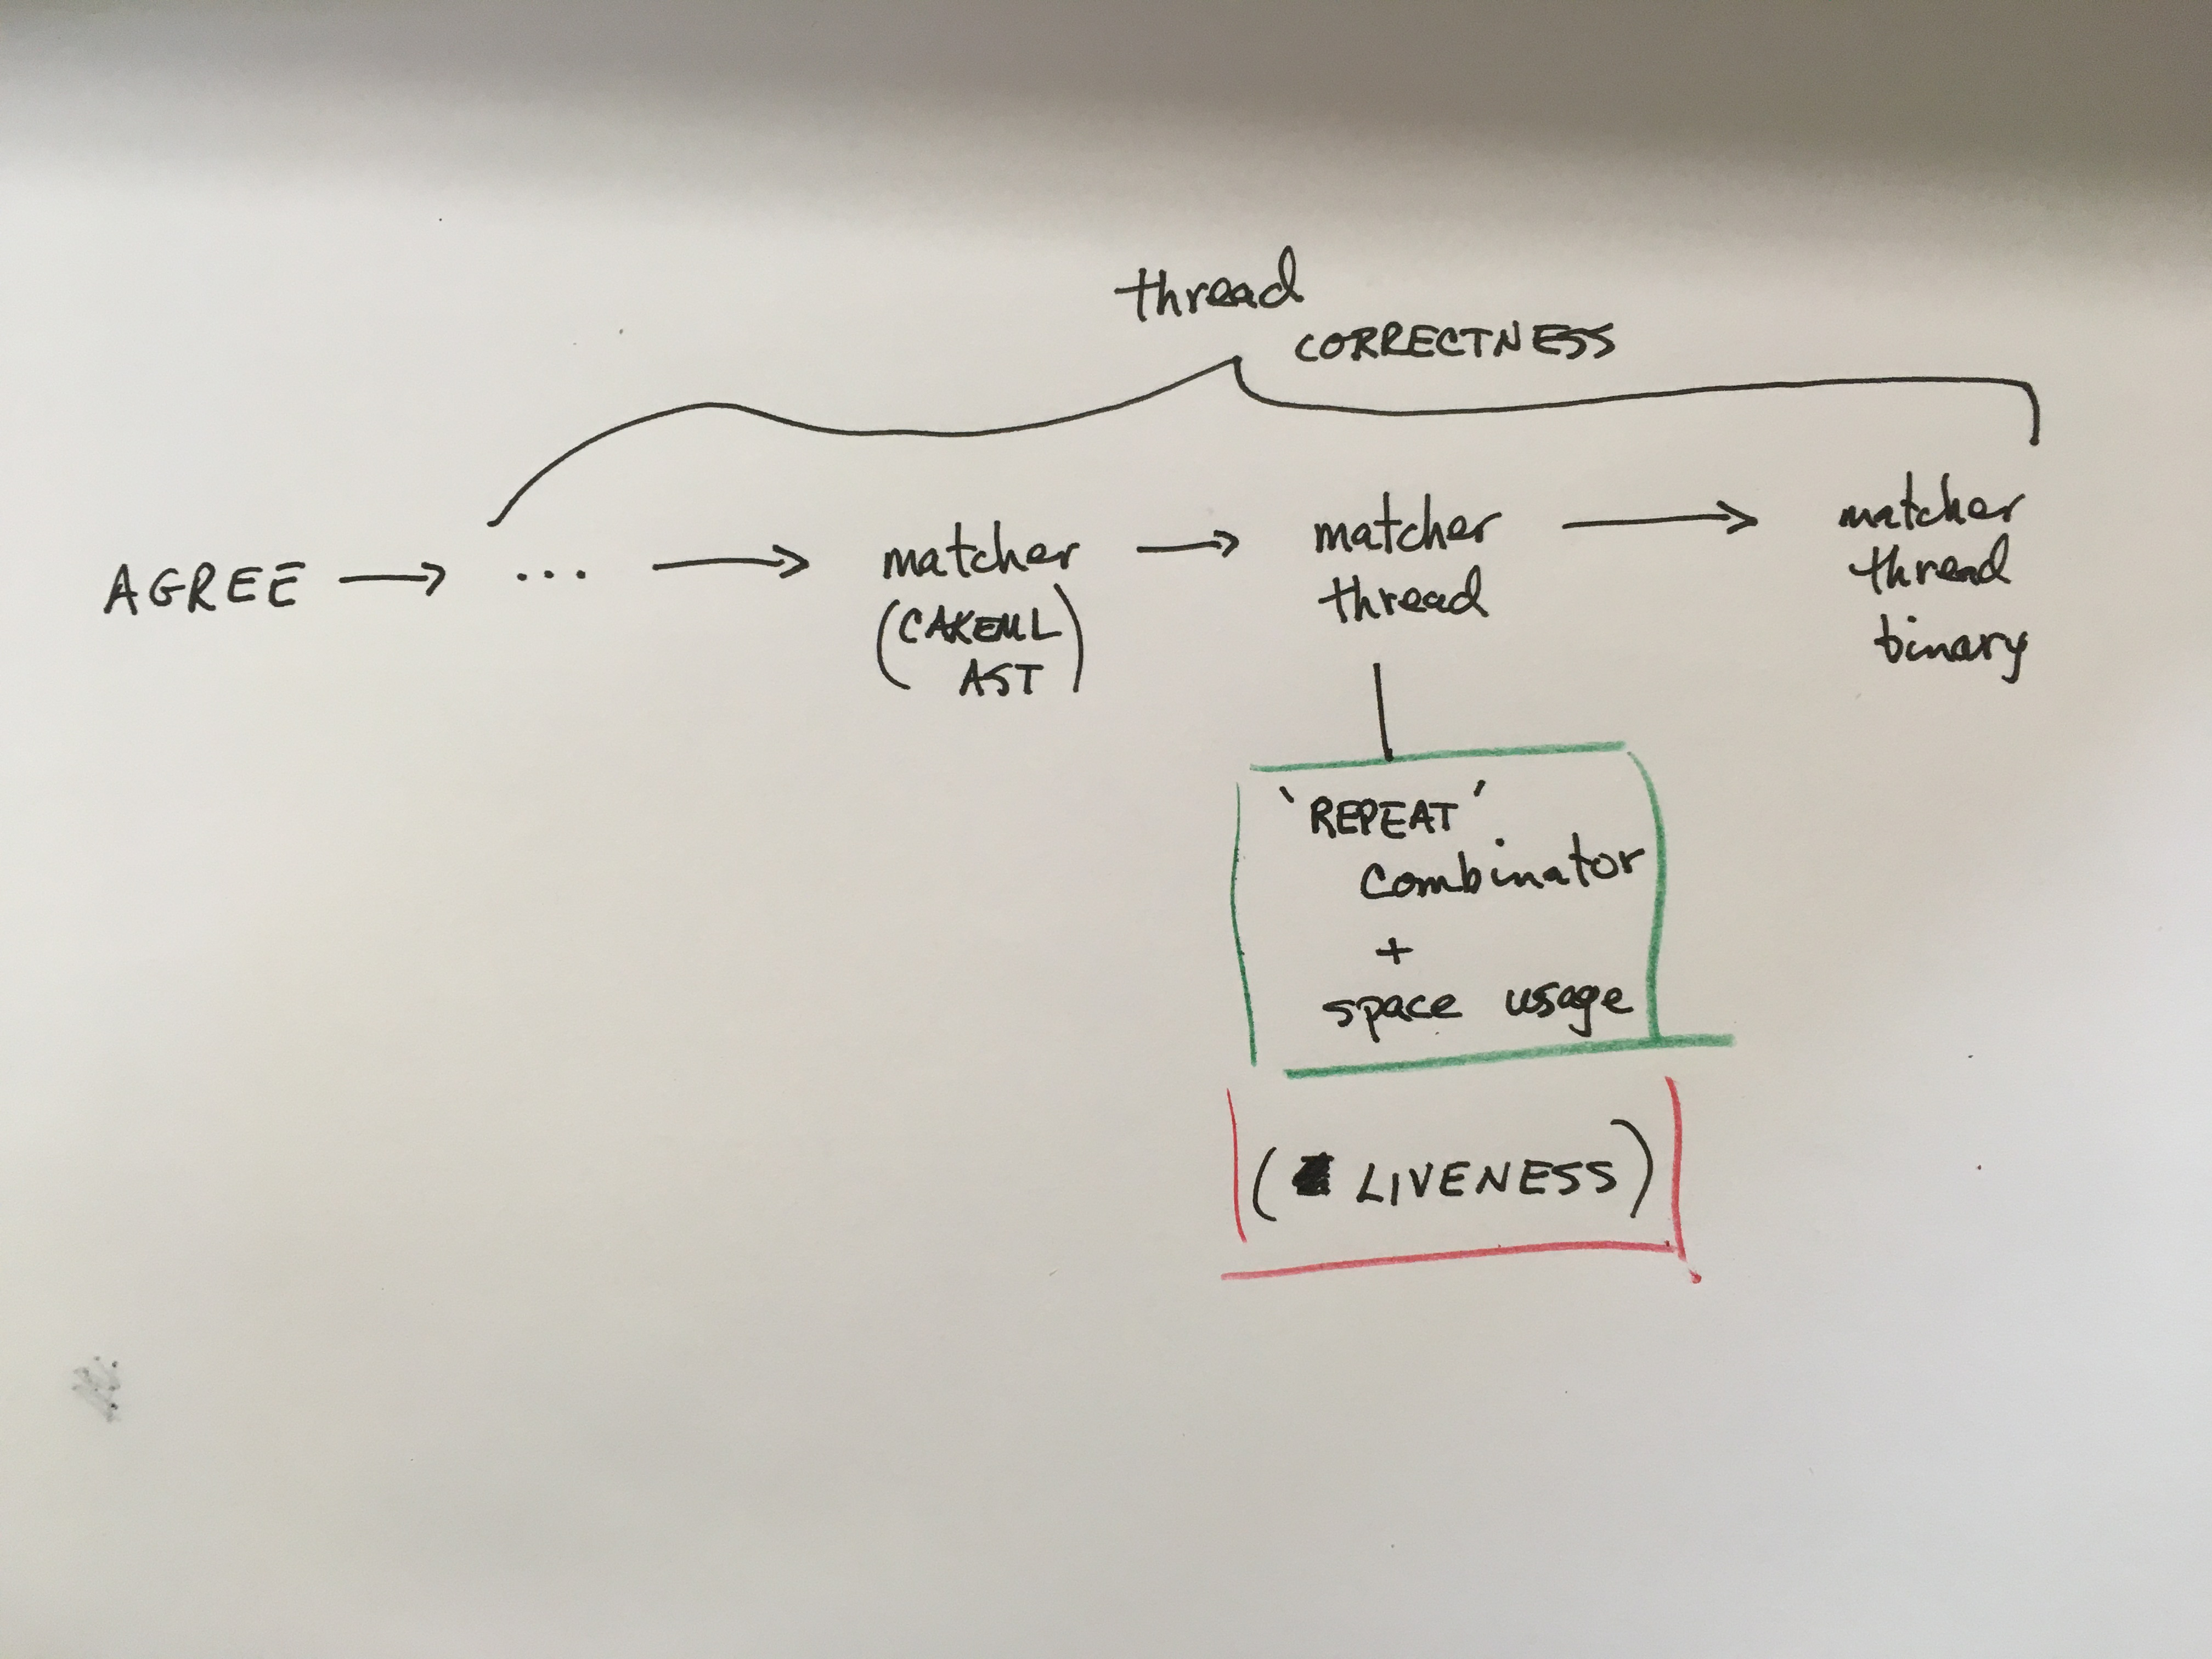
\includegraphics[width=90mm,height=50mm]{thread.jpg}

\end{frame}

\section {Assembling a System Security Case}

\begin{frame}\frametitle{What is the Claim?}

 We have to argue that the newly generated implementations have
 improved the security of the system.

 Current work, so this is somewhat brain-stormy.

\end{frame}


\begin{frame}\frametitle{System-level correctness}

Recall the \textbf{NEAT} acronym on necessary properties for a reference monitor:

\begin{description}[<+->]
\item [\kemph{Non-bypassable}] All paths to target go through RM
\item [\kemph{Evaluable}] testable, verifiable
\item [\kemph{Always invoked}] The RM algorithm is invoked on each and every input
\item [\kemph{Tamper proof}] The RM is not over-writable
\end{description}

\noindent Desirable properties for our implementation! We already `have'

\begin{description}
   \item [Evaluable] (Formal proofs)
   \item [Tamper proof] (seL4 gives isolation)
\end{description}

\end{frame}

\begin{frame}\frametitle{System-level correctness (continued)}

\begin{description}
   \item [Non-bypassable] System-wide property which depends on the
     executable rigorously obeying the boundaries in the model. This
     property depends on the fact that HAMR / seL4 enforces
     architectural boundaries all the way down.

   \item [Always invoked] Does the filter sometimes ignore its input
     and output a stored well-formed element? It shouldn't but how
     could one tell? (Answer: the thread property implies this.)

\end{description}
\end{frame}

\begin{frame}\frametitle{Surveyable system-level correctness with Resolute}

\begin{itemize}
\item For each filter and monitor, the above properties need to be shown and stored.

\item The vast iceberg of the correctness of the security properties
  (in Isabelle/HOL) that seL4 implements need to be brought into the
  picture.

\item For attestation: the toolchain verification story is Coq-based.

\item Disparate evidence supporting our security claim.

\item Our solution: Represent the security argument in Resolute.

\item Goal is \colorbox{orange}{surveyability of the full correctness
  story} for the enhancements generated by the architectural
  transformations

\end{itemize}

\end{frame}


\begin{frame}[fragile]\frametitle{Current and  Future Work}

\begin{itemize}
\item Starting final stage of CASE; CH47 helicopter is our transition platform

\item Trying to raise the level of automation of \konst{SPLAT}

\item Check it out:

\begin{verbatim}
  http://loonwerks.com/projects/case.html
\end{verbatim}

\end{itemize}
\end{frame}

\end{document}
